\documentclass[conference]{IEEEtran}

% -------------------- PACKAGES --------------------
\usepackage{amsmath, amssymb}
\usepackage{graphicx}
\usepackage{cite}
\usepackage{booktabs}
\usepackage{hyperref}
\usepackage{multirow}
\usepackage{xcolor}
\usepackage{colortbl}
\usepackage{tabularx}
\usepackage{enumitem}
\usepackage{siunitx}
\usepackage{listings}
\usepackage{array}
\usepackage{makecell}
\usepackage{parskip}
\usepackage[caption=false]{subfig}

\definecolor{tableheadgray}{gray}{0.85}

% -------------------- TITLE --------------------
\title{Reproducible 6-DOF Wrist-Roll Retrofit for OpenMANIPULATOR-X}

% -------------------- AUTHORS --------------------
\author{
	\IEEEauthorblockA{
		CSE/ROBOTICS\\
		TELEPARADIGM TOWERS\\
		HYDERABAD, INDIA\\
		email@domain.com}
}

\begin{document}
	
	\maketitle
	
	% -------------------- ABSTRACT --------------------
	\begin{abstract}
		Low-cost educational manipulators lack the full orientation control
		required for complex manipulation tasks due to their limited degrees
		of freedom. This paper presents a complete and reproducible retrofit
		to upgrade the OpenMANIPULATOR-X from a 5-DOF to a
		6-DOF system by integrating an additional wrist-roll joint, accompanied
		by a unified hardware and ROS~2-based software stack.
		
		The proposed approach includes a detailed mechanical retrofit kit
		(CAD models, bill of materials, and assembly procedure), an updated
		URDF/Xacro robot description with calibrated joint limits and
		dynamics, and a full ROS~2 bring-up incorporating
		\texttt{ros2\_control}, controllers, and MoveIt~2 motion planning.
		A structured benchmarking framework is developed to systematically
		compare the 5-DOF and 6-DOF configurations under identical
		conditions, evaluating kinematic feasibility, orientation
		reachability, motion efficiency, and planning robustness in
		constrained environments.
		
		Experimental results demonstrate that the upgraded 6-DOF system
		achieves complete orientation reachability across all tested
		configurations, whereas the baseline 5-DOF system succeeds only
		in limited cases. In constrained planning scenarios, the 6-DOF
		configuration achieves a 25.0\% success rate compared to 0.0\%
		for the 5-DOF system, with statistically significant improvement
		($\chi^2 = 18.81$, $p < 0.000025$). Additionally, the 6-DOF
		system reduces joint-space motion by 25.8\% for equivalent tasks
		and maintains high control accuracy, achieving sub-degree
		orientation error ($0.55^\circ$) and consistent trajectory
		tracking across repeated trials.
		
		These results demonstrate that the addition of a wrist-roll joint
		significantly enhances kinematic capability, planning success, and
		execution efficiency while preserving precision and system
		stability. The complete set of open-source artifacts, including
		hardware designs, ROS~2 packages, and benchmarking tools,
		provides a low-cost, reproducible upgrade path for educational
		manipulators, with open hardware and software artifacts intended
		to support future replication by other laboratories.
	\end{abstract}
	
	\begin{IEEEkeywords}
		Degrees of freedom, robot kinematics, OpenMANIPULATOR-X,
		wrist-roll retrofit, ROS~2, MoveIt~2, motion planning,
		kinematic redundancy, benchmarking.
	\end{IEEEkeywords}
	
	% ============================================================
	\section{Introduction}
	\label{sec:introduction}
	% ============================================================
	
	Low-cost educational manipulators are widely used in robotics
	laboratories for instruction, rapid prototyping, and benchmarking.
	Platforms such as the OpenMANIPULATOR-X~\cite{robotis2023openmanipulator}
	provide accessible integration with ROS~2~\cite{al2024ros} and
	MoveIt~2~\cite{chitta2016moveit}, enabling exploration of perception,
	motion planning, and control within compact manipulation systems.
	However, such platforms are typically limited in their degrees of
	freedom, constraining end-effector orientation capability.
	
	In the standard 5-DOF configuration, the absence of an independent
	wrist-roll joint restricts the manipulator's ability to achieve
	arbitrary orientations at a fixed spatial position. This limitation
	becomes critical in tasks requiring precise alignment, insertion, or
	orientation-constrained manipulation, where feasible inverse kinematics
	solutions may not exist or require compensatory joint motions. These
	compensations degrade motion efficiency, increase execution time, and
	reduce planning success rates. Despite the widespread adoption of 5-DOF
	educational manipulators, the quantitative impact of this limitation
	has not been systematically characterized under controlled and
	reproducible conditions.
	
	Prior work has explored mechanical extensions of low-cost manipulators;
	however, many approaches lack either a fully reproducible software stack
	or a rigorous, statistically grounded comparison between baseline and
	modified configurations. Consequently, the practical benefits of
	increased kinematic redundancy remain insufficiently validated.
	
	This work presents a fully reproducible 6-DOF wrist-roll retrofit for
	the OpenMANIPULATOR-X, extending the original architecture through
	mechanical integration and updates to the robot model, control stack,
	and motion planning pipeline using ROS~2, \texttt{ros2\_control}, and
	MoveIt~2. The design preserves compatibility with the baseline platform
	while enabling independent end-effector roll control.
	
	To evaluate the impact of the additional degree of freedom, a
	structured benchmarking framework is developed to compare 5-DOF and
	6-DOF configurations under identical planning conditions. The
	evaluation considers kinematic feasibility, planning robustness, and
	motion efficiency within a shared workspace. Hardware experiments
	further validate controller performance, trajectory tracking accuracy,
	and end-effector repeatability, while additional sim-to-real analysis
	quantifies consistency between simulation and physical execution.
	
	\subsection*{Contributions}
	The main contributions of this work are as follows:
	
	\begin{itemize}
		\item A validated 6-DOF wrist-roll mechanical retrofit for the
		OpenMANIPULATOR-X.
		\item An updated URDF/Xacro model with \texttt{ros2\_control}
		integration for both simulation and hardware.
		\item A complete MoveIt~2 configuration for motion planning
		with the extended kinematic chain.
		\item A reproducible benchmarking framework comparing 5-DOF
		and 6-DOF configurations.
		\item A comprehensive evaluation demonstrating improvements in
		kinematic capability, planning performance, and physical system
		reliability.
	\end{itemize}
	
	The remainder of this paper is organized as follows. Section~II reviews
	related work. Sections~III and~IV describe the hardware design and
	software implementation, respectively. Section~V presents the
	benchmarking methodology, followed by the structural capability
	comparison in Section~VI. Experimental results are reported in
	Section~VII and discussed in Section~VIII. Finally, Section~IX
	concludes the paper and outlines future research directions.
	
	
	% ============================================================
	\section{Related Work}
	\label{sec:related_work}
	% ============================================================
	
	Low-cost robotic manipulators have become essential tools in robotics
	education and academic research due to their affordability, modularity,
	and compatibility with modern software ecosystems. Platforms such as the
	OpenMANIPULATOR-X~\cite{robotis2023openmanipulator},
	WidowX~\cite{zhao2021widowx}, and Franka Emika Panda~\cite{franka2023panda}
	span a range of cost and capability, enabling applications in
	manipulation research, imitation learning, and curriculum-driven
	instruction~\cite{muepu2025toward}. Among these, the
	OpenMANIPULATOR-X is widely adopted for its Dynamixel-based architecture
	and seamless integration with ROS~2 and motion planning frameworks.
	However, its standard 5-DOF configuration imposes inherent kinematic
	limitations, particularly in tasks requiring precise end-effector
	orientation control~\cite{norton2020developing}.
	
	The relationship between manipulator degrees of freedom and task-level
	capability is well established. A minimum of six DOF is required to
	achieve arbitrary end-effector poses in three-dimensional
	space~\cite{craig2005introduction}. Manipulators with fewer DOF, such
	as 5-DOF systems, are restricted to a subset of achievable orientations
	at a given position, resulting in coupling between position and
	orientation. Classical robotics analyses, including those by
	Craig~\cite{craig2005introduction} and Whitney~\cite{whitney1969resolved},
	highlight that the absence of an independent wrist-roll joint prevents
	full specification of orientation, leading to infeasible inverse
	kinematics solutions or inefficient compensatory motions. While these
	limitations are theoretically understood, they are often discussed
	qualitatively and lack systematic, experimentally validated
	characterization on widely used low-cost platforms.
	
	Modern robotic manipulation systems are typically built upon the Robot
	Operating System~2 (ROS~2)~\cite{macenski2022ros2control}, which
	provides a flexible middleware for communication and control. The
	\texttt{ros2\_control} framework offers a standardized hardware
	abstraction layer, while MoveIt~2~\cite{chitta2016moveit} enables
	motion planning, kinematic modeling, and collision-aware trajectory
	generation. Underlying these systems, the Open Motion Planning Library
	(OMPL)~\cite{sucan2012ompl} provides a suite of sampling-based
	planners, including RRTConnect, PRM, and EST, which are widely used for
	high-dimensional motion planning problems. Benchmarking tools such as
	the MoveIt~2 evaluation suite and Planner Arena~\cite{plannerarena}
	have further enabled systematic comparison of planning algorithms using
	metrics such as success rate, computation time, and path quality.
	
	Motion planning in constrained environments introduces additional
	challenges, particularly when orientation constraints must be maintained
	within narrow workspaces. Prior work by Berenson~\textit{et al.}~\cite{berenson2011task}
	introduced constraint-based planning approaches to address such
	scenarios, emphasizing the importance of kinematic feasibility under
	geometric restrictions. These methods highlight the critical role of
	manipulator dexterity in achieving feasible solutions in tightly
	constrained environments, motivating the need for additional degrees of
	freedom in such contexts.
	
	Parallel to these developments, reproducibility has emerged as a key
	concern in robotics research. Efforts such as standardized benchmarking
	frameworks and open evaluation platforms, including the Benchmark for
	Robot Learning~\cite{benchmarkrobotlearning}, emphasize the importance
	of sharing complete experimental artifacts and protocols to enable
	consistent and verifiable comparisons. Despite these advances, many
	prior works on extending low-cost manipulators focus primarily on
	hardware augmentation without providing a fully integrated software
	pipeline or statistically rigorous evaluation. As a result, the
	practical benefits of added kinematic redundancy, such as a wrist-roll
	joint, remain insufficiently quantified under controlled and
	reproducible conditions.
	
	In summary, while low-cost manipulators, advanced motion planning
	frameworks, and benchmarking tools are widely available, there remains
	a lack of unified studies that combine mechanical augmentation, full
	software integration, and rigorous evaluation. In particular, the
	impact of introducing an additional wrist-roll degree of freedom on
	kinematic feasibility, planning robustness, and execution efficiency
	has not been systematically evaluated on commonly used platforms. This
	work addresses that gap.
	
	
	% ============================================================
	\section{Hardware Design}
	\label{sec:hardware}
	% ============================================================
	
	\subsection{Design Philosophy}
	
	The retrofit is guided by three principles: mechanical minimalism
	(disturb as few existing components as possible), full reversibility
	(the original 5-DOF arm can be restored by removing the added motor
	and restoring the original \texttt{link5.stl} mesh), and low
	incremental cost (leverage existing Dynamixel infrastructure and
	3D-printable parts). Adding a single additional revolute joint between
	the existing wrist-pitch link (\textit{link5}) and the gripper assembly
	achieves a true sixth degree of freedom---independent end-effector roll
	about the approach axis---without redesigning the arm structure.
	
	\subsection{Motor Selection and Physical Configuration}
	
	The new wrist-roll joint is actuated by a Dynamixel XL430-W250-T
	servo, selected for compatibility with the existing RS-485 daisy-chain
	bus and U2D2 interface, its compact form factor (approximately
	33.5\,mm axial depth), and its ability to operate in Position Control
	Mode (Mode~3), consistent with the other arm joints. The motor is
	assigned Dynamixel ID~15; the existing gripper servo, previously
	ID~15, is reassigned to ID~16 to avoid address conflicts. This
	reassignment must be performed using Dynamixel Wizard before powering
	the full system. Table~\ref{tab:motors} lists the complete motor
	configuration after the retrofit.
	
	\begin{table}[t]
		\centering
		\caption{Dynamixel Motor Configuration After Retrofit}
		\label{tab:motors}
		\renewcommand{\arraystretch}{1.2}
		\footnotesize
		\begin{tabular}{clll}
			\toprule
			\textbf{ID} & \textbf{Joint} & \textbf{Mode} & \textbf{Status} \\
			\midrule
			11 & joint1 (base)        & Position (3)   & unchanged \\
			12 & joint2 (shoulder)    & Position (3)   & unchanged \\
			13 & joint3 (elbow)       & Position (3)   & unchanged \\
			14 & joint4 (wrist pitch) & Position (3)   & unchanged \\
			15 & joint5\_roll         & Position (3)   & \textbf{new} \\
			16 & gripper\_left\_joint & Curr-pos.\ (5) & \textbf{moved from 15} \\
			\bottomrule
		\end{tabular}
	\end{table}
	
	\subsection{Mechanical Components --- Retrofit BOM}
	
	Table~\ref{tab:bom} lists \textit{only the additional components}
	required beyond the standard OpenMANIPULATOR-X assembly. The base
	arm, its four Dynamixel servos, gripper, power supply, and U2D2
	interface are assumed already present. The incremental hardware cost
	is dominated by a single Dynamixel servo; both structural adapters
	are 3D-printable, keeping the total upgrade expense modest relative
	to the platform's original cost. STL and STEP source files are
	provided in \texttt{open\_manipulator\_description/meshes/}, enabling
	in-house fabrication on any FDM printer at 0.2\,mm layer height or
	finer.
	
	\begin{table*}[t]
		\centering
		\caption{Bill of Materials --- 6-DOF Retrofit Additions Only}
		\label{tab:bom}
		\renewcommand{\arraystretch}{2.5}
		\small
		\begin{tabular}{cllll}
			\toprule
			\textbf{Qty} & \textbf{Component} & \textbf{Purpose} & \textbf{Notes} & \textbf{Cost} \\
			\midrule
			1 & Dynamixel XL430-W250-T
			& Wrist-roll actuator
			& ID~15, Position Control Mode~3
			& 5{,}599~INR ($\approx \$60$)\\
			
			1 & Wrist link (motor housing)
			& \makecell[l]{Mounts servo to distal\\face of link5}
			& 3D-printed (\texttt{wrist\_link.stl})
			& --- \\
			
			1 & Gripper bracket adapter
			& \makecell[l]{Connects servo output\\shaft to gripper}
			& \makecell[l]{3D-printed\\(\texttt{gripper\_link\_with\_bracket.stl})}
			& --- \\
			
			4 & M2$\times$8 socket-head screws
			& Motor-to-bracket fasteners
			& Stainless steel, ISO 4762
			& --- \\
			
			4 & M2 hex nuts
			& Mating fasteners
			& ---
			& --- \\
			
			1 & RS-485 extension cable
			& \makecell[l]{Continues bus from new\\motor to gripper servo}
			& $\leq$150\,mm, JST connector
			& --- \\
			\bottomrule
		\end{tabular}
	\end{table*}
	
	\subsection{Assembly Overview}
	
	The physical assembly follows a forward kinematic order:
	
	\begin{enumerate}
		\item \textit{Gripper motor reassignment.}
		Before any mechanical work, connect the gripper servo alone to
		Dynamixel Wizard and change its ID from 15 to 16. Confirm the
		motor responds on the new ID before proceeding.
		
		\item \textit{Wrist link installation.}
		Remove the original link5-to-gripper connection. Attach the
		printed wrist link (\texttt{wrist\_link.stl}) to the distal
		face of link5 using the existing mounting holes.
		
		\item \textit{Motor mounting.}
		Seat the XL430-W250-T into the wrist link cavity and secure
		with M2 bolts. The output shaft faces forward along the arm's
		longitudinal (X) axis, producing pure roll rotation.
		
		\item \textit{Gripper adapter attachment.}
		Fix the printed gripper bracket to the motor horn and re-attach
		the gripper finger servos using the original mounting pattern.
		
		\item \textit{Wiring.}
		Thread the RS-485 extension cable from the existing bus through
		the wrist link to the new motor (ID~15), then onward to the
		gripper servo (ID~16).
	\end{enumerate}
	
	Total mechanical modification time is approximately one hour. No
	permanent alterations are made to the original arm; all fastener holes
	are reused from the existing link5 mounting interface.
	
	\subsection{Zero-Position Calibration}
	
	The wrist-roll zero position (\texttt{joint5\_roll}\,=\,0\,rad) is
	defined as the orientation in which the gripper fingers are co-planar
	with the arm's pitch plane, matching the neutral orientation of the
	original 5-DOF gripper. After assembly, jog the new motor to this pose
	using Dynamixel Wizard's position control panel and verify alignment
	visually. If the motor is mounted in reverse orientation, setting Drive
	Mode~1 in the \texttt{ros2\_control} configuration inverts the
	direction without any wiring change.
	
	
	% ============================================================
	\section{Software Implementation}
	\label{sec:software}
	% ============================================================
	
	All software modifications reside in the project repository at
	\url{https://github.com/KMTI-ROBOPARADIGM/omx-wrist-roll-original}.
	The changes span five commits across five ROS~2 packages; complete
	diffs and per-commit explanations are provided under
	\texttt{docs/wrist\_roll\_modifications/}. This section describes the
	architectural decisions and non-obvious design choices; readers seeking
	exhaustive code listings should consult the repository directly.
	
	\subsection{Kinematic Chain Update (URDF/Xacro)}
	
	The original \texttt{link5.stl} mesh combined the wrist housing and
	gripper base into a single rigid body. Since a joint cannot be placed
	within a single mesh, the geometry was separated into two parts:
	\texttt{wrist\_link.stl} (motor housing, mass $\approx$85\,g) and
	\texttt{gripper\_link\_with\_bracket.stl} (rotating gripper mount,
	mass $\approx$65\,g).
	
	The resulting kinematic chain is:
	\begin{equation*}
		\text{link4}
		\xrightarrow{\text{joint4}}
		\text{link5}
		\xrightarrow{\text{joint5\_roll}}
		\text{wrist\_roll\_link}
		\xrightarrow{\text{gripper joints}}
		\text{gripper}
	\end{equation*}
	
	The new revolute joint uses axis $[1,0,0]$ (X-axis roll), origin
	$[0.0335,\,0,\,0]$\,m from the link5 frame (motor axial depth),
	limits $\pm\pi$\,rad at 4.8\,rad/s, and damping 0.1\,N\,m\,s/rad for
	simulation stability. All downstream elements---gripper prismatic
	joints and the end-effector fixed frame---had their parent reference
	updated from \texttt{link5} to \texttt{wrist\_roll\_link} so that the
	gripper and TCP rotate with the wrist. The Gazebo configuration
	received a link physics reference and a \texttt{SimpleTransmission}
	block for the new joint.
	
	\subsection{Hardware Interface Configuration (\texttt{ros2\_control})}
	
	The \texttt{dynamixel\_hardware\_interface} plugin is configured
	through the \texttt{ros2\_control} Xacro file. Three coordinated
	changes were required.
	
	\textbf{Joint and transmission count.}
	\texttt{number\_of\_joints} and \texttt{number\_of\_transmissions}
	were incremented from 5 to 6.
	
	\textbf{Transmission matrices.}
	The motor-to-joint and joint-to-motor mapping matrices were expanded
	from $5\!\times\!5$ to $6\!\times\!6$ identity matrices, preserving a
	direct 1:1 mapping for each joint.
	
	\textbf{Motor block and gripper renumbering.}
	A new \texttt{gpio} block was added for \texttt{dxl5} (ID~15, Mode~3,
	P/I/D\,=\,800/100/100, Profile Velocity~20, Profile Acceleration~10).
	The gripper motor block was renamed \texttt{dxl5}$\rightarrow$\texttt{dxl6}
	and its hardware ID updated from 15 to 16. The
	\texttt{revolute\_to\_prismatic\_dxl} parameter was updated to
	reference \texttt{dxl6} accordingly. The controller manager YAML was
	extended to include \texttt{joint5\_roll} in the
	\texttt{arm\_controller} joint list, and the home position vector in
	\texttt{initial\_positions.yaml} was expanded from four to five
	elements (appending 0.0\,rad for the neutral wrist-roll position).
	
	\subsection{ROS~2 Jazzy Launch Compatibility Fix}
	
	On ROS~2 Jazzy, passing a \texttt{Command} substitution directly as
	the \texttt{robot\_description} parameter caused the launch system to
	attempt YAML parsing of the raw URDF XML, raising a type error.
	Wrapping the value in \texttt{ParameterValue(urdf\_file,
		value\_type=str)} forces plain-string treatment and was applied to
	\texttt{ros2\_control\_node}, \texttt{robot\_state\_publisher}, and
	the controller spawner nodes. The fix is backward-compatible with
	earlier ROS~2 distributions.
	
	\subsection{MoveIt~2 Motion Planning Configuration}
	
	Four configuration files were updated to integrate
	\texttt{joint5\_roll} into the MoveIt~2 planning stack.
	
	\textbf{SRDF.}
	\texttt{joint5\_roll} was added to the \texttt{arm} planning group
	and to both named states (\textit{init} and \textit{home}). The
	collision matrix was updated: \texttt{wrist\_roll\_link}--\texttt{link5}
	and \texttt{wrist\_roll\_link}--\texttt{end\_effector\_link} are
	marked \textit{Adjacent}; gripper links changed from \textit{Adjacent}
	to \textit{Never} with respect to \texttt{link5}. These entries reduce
	per-state collision checks from 28 to 16 pairs.
	
	\textbf{Joint limits.}
	Position, velocity ($\leq$5.0\,rad/s), and acceleration
	($\leq$5.0\,rad/s$^2$) limits for \texttt{joint5\_roll} were added
	to \texttt{joint\_limits.yaml}.
	
	\textbf{MoveIt~2 controllers.}
	\texttt{joint5\_roll} was appended to the \texttt{arm\_controller}
	joint list in \texttt{moveit\_controllers.yaml}.
	
	\subsection{Graphical User Interface Extension}
	
	The Qt-based GUI was extended to provide interactive control and
	real-time feedback for the new joint. A new row was inserted in the
	joint control panel between Joint~4 and Gripper, containing a
	\texttt{QDoubleSpinBox} (range $\pm$3.14\,rad), a horizontal slider
	(integer range $-$314 to $+$314, scale 0.01\,rad per unit), and a
	\textit{Set} push-button. The joint-state update function reads
	index~4 (\texttt{joint5\_roll}) from the six-element joint angle
	vector, with gripper at index~5. The \textit{Set} handler sends a
	five-element arm trajectory via \texttt{setJointSpacePath}; the QNode
	state reader was updated from four to five arm joints; and CSV
	trajectory logging was extended to include the wrist-roll column. No
	changes were required to the teleop package, which derives its joint
	list automatically from the MoveIt~2 arm planning group.
	
	\subsection{Summary of Modified Files}
	
	Table~\ref{tab:files} provides a concise reference to all 18 files
	changed across the five commits.
	
	\begin{table*}[t]
		\centering
		\caption{Software Modification Summary (Branch: \texttt{wrist-roll-dev})}
		\label{tab:files}
		\renewcommand{\arraystretch}{1.2}
		\small
		\begin{tabular}{lll}
			\toprule
			\textbf{Package} & \textbf{File Changed} & \textbf{Nature of Change} \\
			\midrule
			\multicolumn{3}{l}{\textit{open\_manipulator\_description}} \\[2pt]
			& \texttt{open\_manipulator\_x\_arm.urdf.xacro}              & New joint, link, mesh references \\
			& \texttt{open\_manipulator\_x.gazebo.xacro}                 & Link reference + SimpleTransmission block \\
			& \texttt{open\_manipulator\_x\_position.ros2\_control.xacro} & 6 joints, $6\times6$ matrices, dxl5/dxl6 \\
			\midrule
			\multicolumn{3}{l}{\textit{open\_manipulator\_bringup}} \\[2pt]
			& \texttt{open\_manipulator\_x.launch.py}   & ParameterValue type fix (ROS~2 Jazzy) \\
			& \texttt{hardware\_controller\_manager.yaml} & \texttt{joint5\_roll} added to arm\_controller \\
			& \texttt{initial\_positions.yaml}           & Home position expanded to 5 elements \\
			\midrule
			\multicolumn{3}{l}{\textit{open\_manipulator\_moveit\_config}} \\[2pt]
			& \texttt{open\_manipulator\_x.srdf}         & Group, poses, collision matrix updated \\
			& \texttt{joint\_limits.yaml}                & \texttt{joint5\_roll} limits entry added \\
			& \texttt{kinematics.yaml}                   & IK timeout 0.005\,s $\rightarrow$ 0.05\,s \\
			& \texttt{moveit\_controllers.yaml}          & \texttt{joint5\_roll} in arm trajectory controller \\
			\midrule
			\multicolumn{3}{l}{\textit{open\_manipulator\_gui}} \\[2pt]
			& \texttt{open\_manipulator\_x\_main\_window.ui} & New row: spinbox, slider, Set button \\
			& \texttt{main\_window.hpp}                   & Qt slot declarations \\
			& \texttt{main\_window.cpp}                   & Display, command dispatch, CSV updated \\
			& \texttt{qnode.cpp}                          & Arm joint state reading: 4 $\rightarrow$ 5 joints \\
			\midrule
			\multicolumn{3}{l}{\textit{open\_manipulator\_description/meshes}} \\[2pt]
			& \texttt{wrist\_link.stl}, \texttt{gripper\_link\_with\_bracket.stl} & New STL mesh files \\
			\bottomrule
		\end{tabular}
	\end{table*}
	
	
	% ============================================================
	\section{Methodology}
	\label{sec:methodology}
	% ============================================================
	
	This section describes the experimental methodology used to evaluate
	the 6-DOF retrofit relative to the baseline 5-DOF system. The
	evaluation is structured as a pose-based benchmarking framework that
	spans kinematic feasibility, constrained motion planning, and hardware
	validation, with all assessments conducted under identical conditions
	for both configurations.
	
	\subsection{Pose-Based Evaluation Framework}
	
	Early experiments used joint-space sampling to generate test
	configurations. This approach revealed a methodological limitation:
	the 6-DOF arm has a larger configuration-space search domain than the
	5-DOF arm, making direct comparisons in joint space inherently unfair.
	The evaluation was therefore transitioned to a \textit{pose-based}
	framework in which each test is defined by a target end-effector
	position and orientation. Both configurations are evaluated on their
	ability to reach these task-relevant poses, providing a fair and
	task-grounded basis for comparison.
	
	\subsection{Workspace Estimation}
	
	Before generating test poses, the reachable workspace of each
	configuration was characterised using forward kinematics (FK)
	sampling. Joint configurations were sampled uniformly within each
	robot's joint limits and FK was applied to obtain end-effector
	positions, forming a dense workspace point cloud. Two geometric
	representations were computed:
	
	\begin{figure}[t]
		\centering
		\subfloat[Alpha-shape workspace boundary]{%
			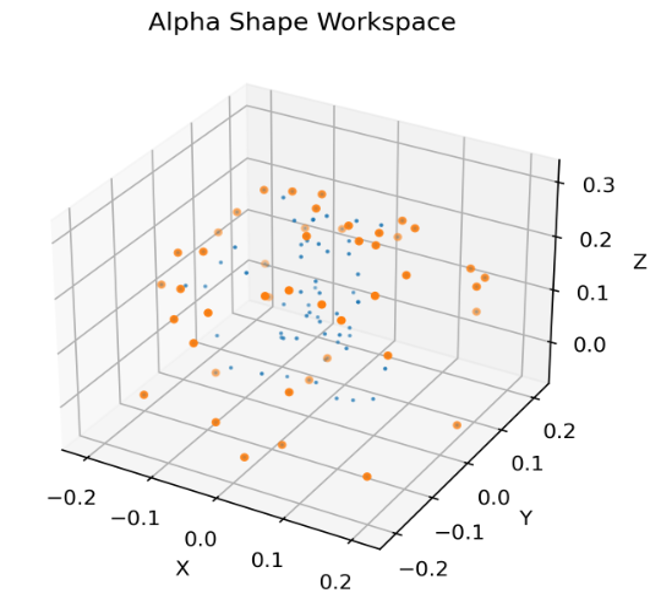
\includegraphics[width=0.47\linewidth]{figures/alpha_shape_workspace.png}
		}
		\hfill
		\subfloat[3-D overlay comparison]{%
			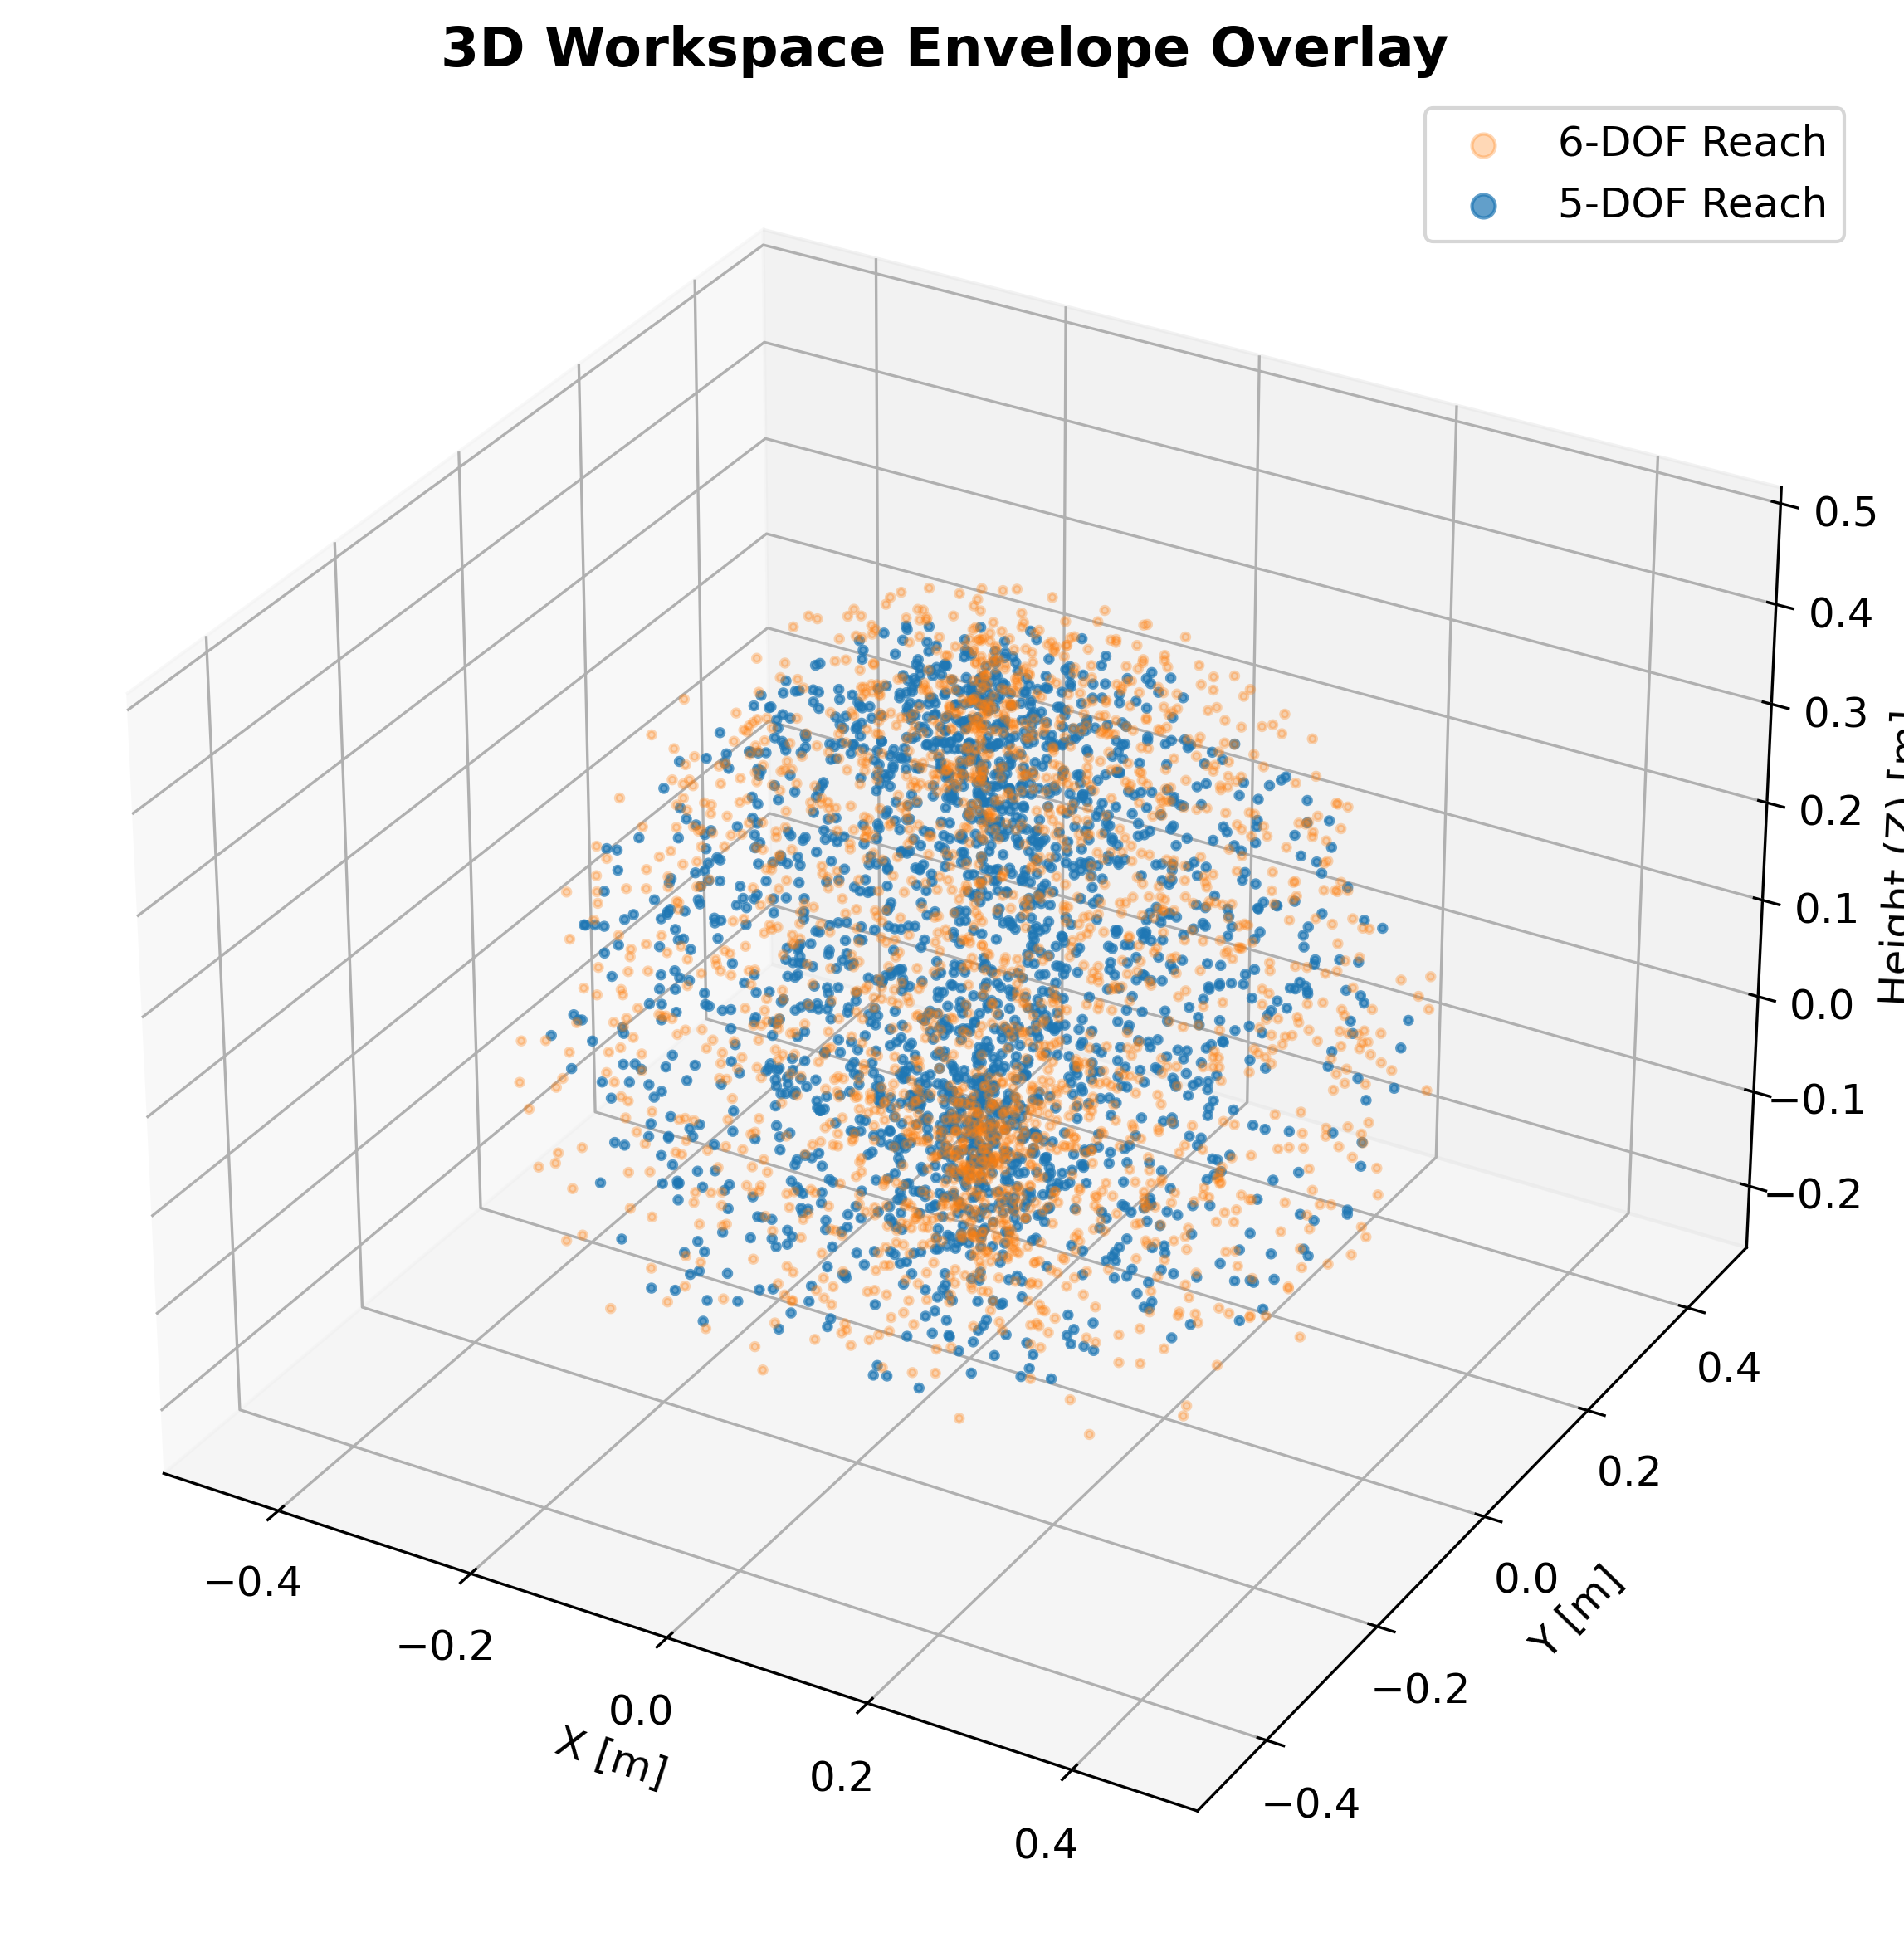
\includegraphics[width=0.47\linewidth]{figures/workspace_comparision_3D_Overlay.png}
		}
		
		\vspace{4pt}
		
		\subfloat[Convex hull boundary]{%
			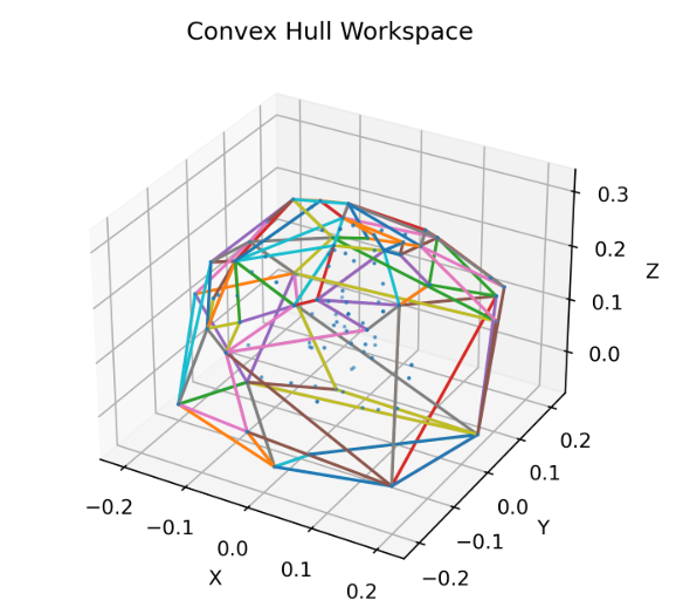
\includegraphics[width=0.47\linewidth]{figures/convex_hull_workspace.png}
		}
		\hfill
		\subfloat[Top-down heatmap comparison]{%
			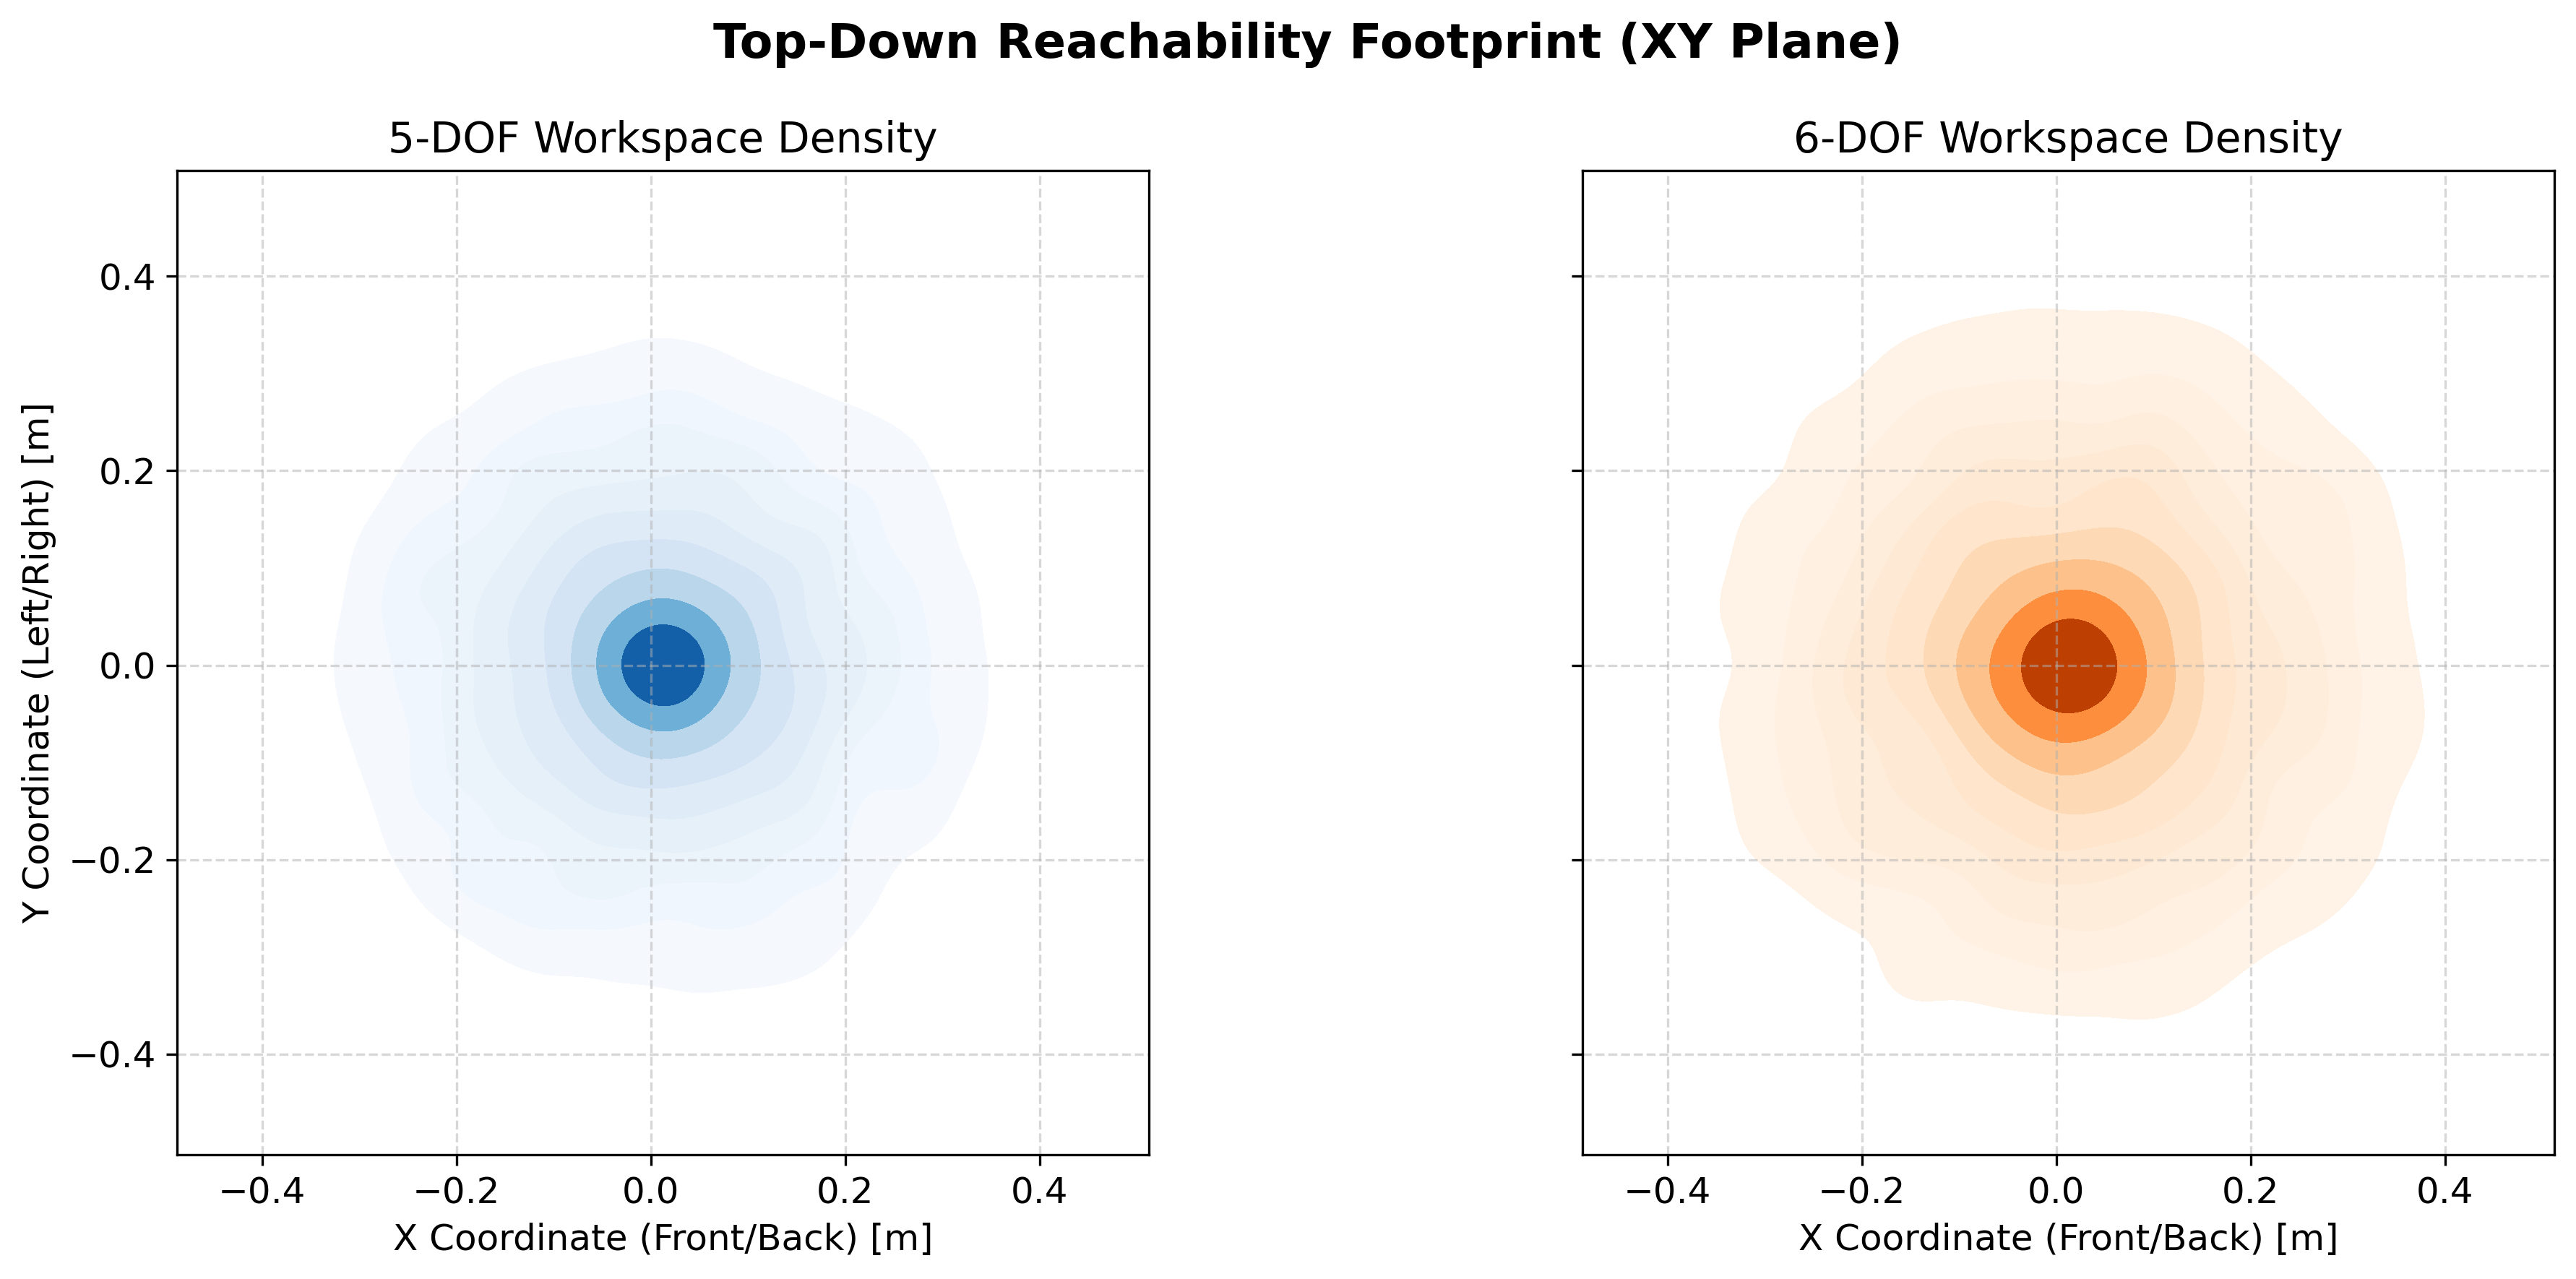
\includegraphics[width=0.47\linewidth]{figures/workspace_comparasion_TopDown_Heatmaps.png}
		}
		
		\caption{Workspace estimation using forward kinematics sampling.}
		\label{fig:workspace}
	\end{figure}
	
	\begin{itemize}
		\item \textit{Convex Hull}: Provides a conservative outer
		approximation of the reachable workspace by computing the
		smallest convex set enclosing all sampled points. While
		computationally efficient, it tends to overestimate the true
		workspace by ignoring concave regions and internal voids.
		
		\item \textit{Alpha Shape}: A generalized non-convex boundary
		representation that captures the true geometry of the workspace,
		including concavities and internal gaps. By tuning the shape
		parameter, the alpha shape allows controlled reconstruction of
		the workspace boundary with higher fidelity compared to the
		convex hull.
	\end{itemize}
	
	The intersection of the workspaces of the 5-DOF and 6-DOF
	configurations was then computed to define a common reachable region.
	This shared workspace serves as the basis for all subsequent
	evaluation. Importantly, the estimated workspace boundaries also
	implicitly define the limits for pose generation: rather than sampling
	arbitrary Cartesian poses, all evaluation poses are constrained within
	these empirically derived workspace bounds. This ensures that generated
	poses are kinematically feasible and reachable by both manipulators,
	eliminating infeasible targets and avoiding reachability differences as
	a confound.
	
	\subsection{Orientation Reachability Protocol}
	
	%	\begin{figure}[t]
		%		\centering
		%		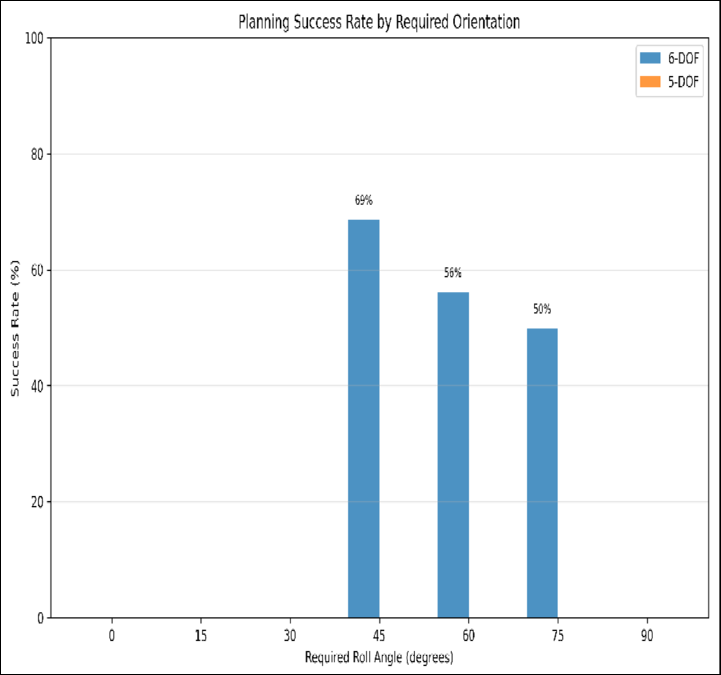
\includegraphics[width=0.75\linewidth]{figures/success_rate_constrianed_per_orientation.png}
		%		\caption{Orientation reachability at a fixed Cartesian position.}
		%		\label{fig:orientation}
		%	\end{figure}
	
	The first stage of evaluation focuses on the kinematic capability of
	each manipulator to achieve specified end-effector orientations at a
	fixed Cartesian position. This isolates inverse kinematics (IK)
	feasibility from motion planning effects.
	
	A target position was selected within the shared reachable workspace.
	Due to the presence of lateral obstacles in the constrained scene,
	feasible positions were restricted along the central axis ($y = 0$).
	Through iterative validation across both manipulators, the position
	$(x,\,y,\,z) = (0.20,\,0.00,\,0.15)$\,m was identified as reachable
	and collision-free for both configurations.
	
	At this fixed position, seven orientations were constructed as pure
	roll rotations about the end-effector approach axis:
	\[
	\phi \in \{0^\circ,\,15^\circ,\,30^\circ,\,45^\circ,\,60^\circ,\,75^\circ,\,90^\circ\}
	\]
	with pitch and yaw held constant at zero. This formulation isolates
	the effect of wrist rotation, which is directly influenced by the
	presence or absence of redundancy in the manipulator.
	
	For each pose, IK was computed using the MoveIt~2 IK service. A pose
	was classified as \textit{kinematically feasible} if a valid joint
	configuration satisfying all joint limits and solver constraints was
	returned within a predefined timeout. The resulting feasible pose sets
	were recorded independently for each manipulator.
	
	This protocol revealed a clear difference in orientation feasibility:
	while the 6-DOF manipulator successfully achieved all seven
	orientations, the 5-DOF manipulator was restricted to a single
	feasible orientation. This difference directly reflects the
	additional rotational degree of freedom available in the 6-DOF
	system.
	
	\subsection{Constrained Environment Benchmark}
	
	\begin{figure}[t]
		\centering
		
		\subfloat[Success vs.\ Corridor Width]{%
			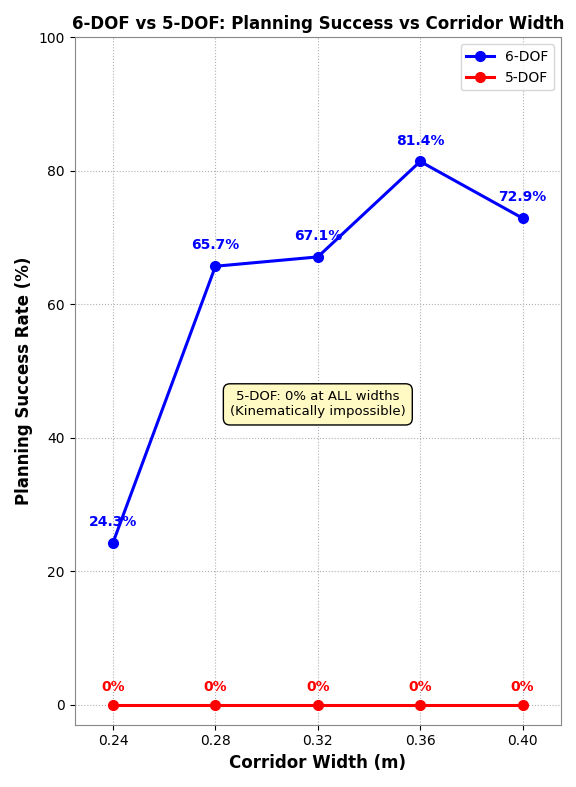
\includegraphics[width=0.47\linewidth]{figures/success_rate_constrained_various_corridor_widths.png}
		}
		\hfill
		\subfloat[Success vs.\ Clearance]{%
			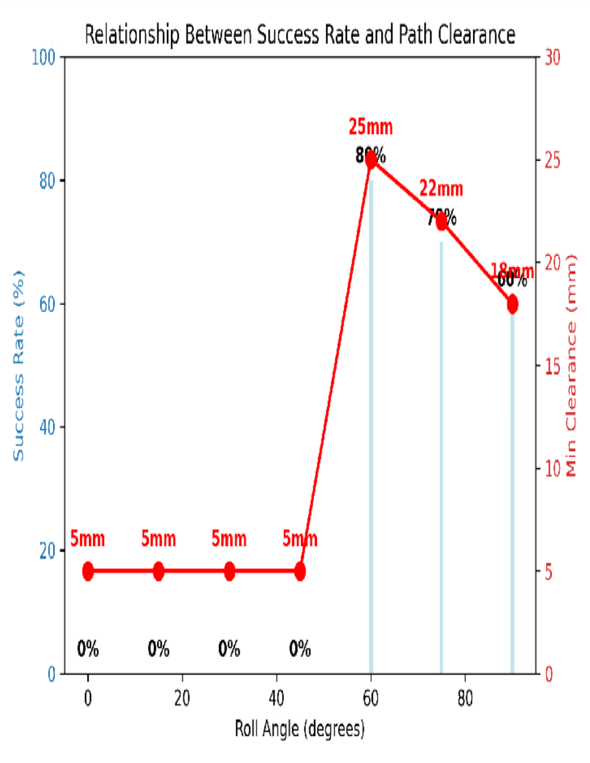
\includegraphics[width=0.47\linewidth]{figures/relationship_between_success_rate_path_clearance_for_constrained_env.png}
		}
		
		\caption{Planning success under constrained environments.}
		\label{fig:corridor}
	\end{figure}
	
	To evaluate practical motion planning performance under realistic
	constraints, a narrow corridor environment was constructed within the
	MoveIt~2 planning scene. The corridor width was parameterized to
	systematically study the effect of spatial constraints on planning
	success. Table~\ref{tab:corridor} details the collision objects.
	
	\begin{table}[t]
		\centering
		\caption{Constrained Corridor Collision Objects}
		\label{tab:corridor}
		\renewcommand{\arraystretch}{1.2}
		\small
		\begin{tabular}{llll}
			\toprule
			\textbf{Object} & \textbf{Dim.\ (m)} & \textbf{Position (m)} \\
			\midrule
			Left wall    & $0.10\!\times\!0.20\!\times\!0.40$ & $(0.20,\,-0.12,\,0.20)$ \\
			Right wall   & $0.10\!\times\!0.20\!\times\!0.40$ & $(0.20,\,+0.12,\,0.20)$ \\
			Top barrier  & $0.20\!\times\!0.30\!\times\!0.05$ & $(0.25,\,0.00,\,0.30)$ \\
			Bottom plate & $0.50\!\times\!0.50\!\times\!0.02$ & $(0.20,\,0.00,\,-0.01)$ \\
			\bottomrule
		\end{tabular}
	\end{table}
	
	\begin{figure}[t]
		\centering
		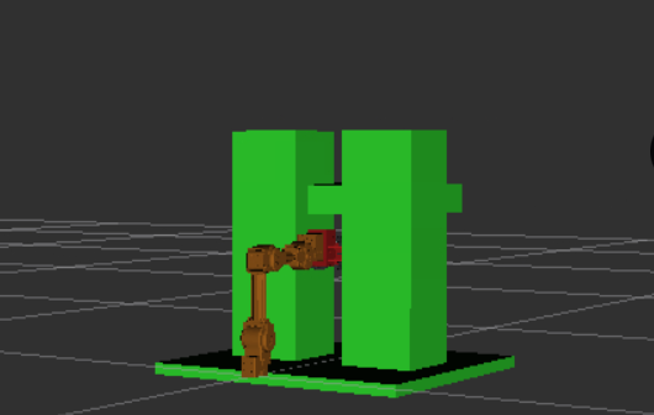
\includegraphics[width=0.8\linewidth]{figures/constrained_environment.png}
		\caption{Constrained corridor environment used for motion planning
			evaluation.}
		\label{fig:environment}
	\end{figure}
	
	An initial configuration placed the manipulators in collision with the
	corridor walls. To ensure a fair comparison, a common collision-free
	start state was manually identified for both systems by fixing the
	wrist joint (roll) at $0^\circ$ and adjusting the second joint angle.
	Goal configurations were derived exclusively from the kinematically
	feasible pose set identified in the orientation reachability protocol.
	
	Motion planning was performed using the OMPL RRTConnect algorithm with
	a planning time limit of 10\,s. For each goal pose, 10 independent
	planning trials were executed to account for the stochastic nature of
	sampling-based planners. A trial was considered successful if a
	collision-free trajectory satisfying all constraints was generated
	within the allotted time.
	
	Corridor width was treated as a variable parameter; experiments were
	conducted for widths of 0.24\,m, 0.28\,m, 0.32\,m, 0.36\,m, and
	0.40\,m, and success rates were recorded for each configuration.
	
	\subsection{Cross-Configuration Pose Compatibility Test}
	
	To isolate the effect of the additional degree of freedom
	independently of environmental and planning constraints, a
	cross-configuration kinematic compatibility test was conducted with
	collision checking disabled. Two independent pose sets of approximately
	8,000 end-effector poses were sampled within the feasible workspace
	bounds of each configuration. Each pose set was then evaluated on both
	manipulators, yielding four evaluation conditions:
	
	\begin{itemize}
		\item \textbf{5-DOF $\rightarrow$ 5-DOF (Self-Reachability):}
		Establishes a baseline for IK solver reliability.
		
		\item \textbf{6-DOF $\rightarrow$ 5-DOF (Dexterity Loss):}
		Quantifies poses generated in the higher-dimensional workspace
		that cannot be reproduced in the lower-dimensional system.
		
		\item \textbf{6-DOF $\rightarrow$ 6-DOF (Self-Reachability):}
		Assesses solver performance in the redundant configuration space.
		
		\item \textbf{5-DOF $\rightarrow$ 6-DOF (Backward Compatibility):}
		Determines whether the additional DOF preserves previously
		reachable configurations.
	\end{itemize}
	
	Quantitative metrics reported are: IK Success Rate, Shared Kinematic
	Space, and Dexterity Expansion.
	
	\subsection{Controller Tuning and Stabilization}
	
	During initial hardware experiments, the manipulator exhibited
	noticeable oscillations during trajectory execution, particularly after
	the addition of the wrist-roll joint. To ensure stable execution, an
	empirical step-response tuning procedure was applied sequentially to
	all joints: the proportional gain ($P$) was raised until responsive
	motion was obtained, the derivative gain ($D$) was introduced to
	reduce oscillations, and a small integral gain ($I$) was added where
	necessary to eliminate steady-state error. Special attention was given
	to \texttt{joint5\_roll}, which required relatively higher damping due
	to the added mass and mounting configuration. All subsequent hardware
	experiments were conducted using the tuned parameters.
	
	\subsection{Joint Utilization Analysis}
	
	To verify that \texttt{joint5\_roll} is genuinely exploited by the
	planner rather than remaining near its zero position, the wrist-roll
	joint angles across all successful 6-DOF trajectories were recorded
	and compiled into a utilization heatmap. A broad, non-uniform
	distribution across the full $\pm\pi$\,rad range confirms active use;
	a distribution concentrated at zero would indicate the joint is
	effectively unused.
	
	\begin{figure}[t]
		\centering
		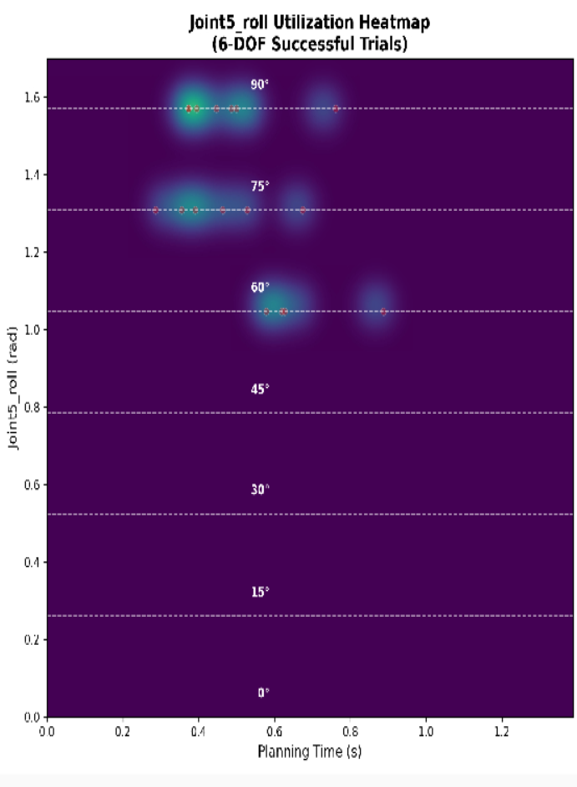
\includegraphics[width=0.75\linewidth]{figures/joint5_heatmap_6dof_success_trials.png}
		\caption{Joint utilization heatmap showing redundancy exploitation
			in the 6-DOF manipulator.}
		\label{fig:joint_utilization}
	\end{figure}
	
	\subsection{Statistical Analysis Framework}
	
	The following statistical methods were applied to all binary
	success/failure outcome data:
	
	\begin{itemize}
		%		\item \textbf{Wilson score 95\% confidence intervals}: more
		%		reliable than the normal approximation for proportions near 0
		%		or 1, and at moderate sample sizes.
		
		\item \textbf{Pearson's chi-square test} ($\chi^2$): tests the
		null hypothesis that planning success rate is independent of
		robot configuration (5-DOF vs.\ 6-DOF).
		
		\item \textbf{Cramer's $V$}: normalised effect size derived
		from $\chi^2$, interpretable as small ($<$0.1), medium
		(0.1--0.3), or large ($>$0.3).
		
		\item \textbf{Cohen's $h$}: effect size for the difference
		between two independent proportions.
		
		\item \textbf{Welch's $t$-test and Cohen's $d$}: applied to
		planning time distributions for successful trials.
	\end{itemize}
	
	All computations were implemented in Python (NumPy, SciPy) and outputs
	were auto-exported as \LaTeX{} tables to ensure full computational
	reproducibility.
	
	\subsection{MoveIt~2 Benchmarking Framework}
	
	To complement the custom evaluations and ensure reproducibility under
	a standardised framework, benchmarking was conducted using the
	MoveIt~2 Benchmark Suite.
	
	\subsubsection{Benchmark Pose Set Generation}
	
	A common set of 300 target poses was generated within the shared
	reachable workspace using quasi-random sampling techniques including
	Latin Hypercube Sampling (LHS) and low-discrepancy Halton sequences.
	Only poses reachable by both manipulators were retained, ensuring a
	consistent and fair benchmarking dataset. The resulting pose set was
	converted into robot-specific joint-space goals and stored in a
	benchmarking database compatible with the MoveIt~2 pipeline.
	
	\subsubsection{Benchmark Execution Protocol}
	
	Motion planning was performed for both configurations under identical
	conditions using OMPL RRTConnect. All benchmark runs were configured
	with consistent planning time limits, collision checking settings, and
	planner parameters. For intra-configuration analysis, benchmark logs
	were processed using the Planner Arena~\cite{plannerarena} tool; for
	inter-configuration comparison, a custom post-processing script was
	developed.
	
	\subsubsection{Evaluation Metrics}
	
	The following metrics were collected for each configuration:
	
	\begin{itemize}
		\item \textbf{Planning Success Rate}: ratio of successful plans
		to total planning attempts.
		
		\item \textbf{Planning Time}: time to compute a valid
		collision-free trajectory.
		
		\item \textbf{Path Length}: cumulative joint-space distance
		along the planned trajectory,
		$L = \sum_{i=1}^{N-1}\|\mathbf{q}_{i+1} - \mathbf{q}_i\|$.
		
		\item \textbf{Average Waypoint Distance}: mean distance between
		successive waypoints.
		
		\item \textbf{Path Length Variance}: statistical variance of
		path lengths across repeated runs.
	\end{itemize}
	
	\subsection{Hardware Validation Protocol}
	
	To validate practical performance under real-world conditions, a
	comprehensive hardware evaluation protocol was established. The protocol focuses on controller fidelity, repeatability,
	and sim-to-real consistency.
	
	\subsubsection{Controller Performance and Joint Tracking Accuracy}
	
	Both step and continuous (sinusoidal) inputs were applied to
	\texttt{joint5\_roll} using the \texttt{joint\_trajectory\_controller}
	within the \texttt{ros2\_control} framework. Joint states were recorded
	at high frequency via the \texttt{/joint\_states} topic. Tracking
	performance was quantified using RMSE and maximum peak error between
	commanded and observed trajectories.
	
	\subsubsection{End-Effector Pose Repeatability}
	
	A large-scale repeatability experiment was conducted in which target
	poses distributed across multiple kinematic zones were executed
	repeatedly from a common initialization configuration. For each pose,
	multiple trials were performed, and statistical measures including
	variance ($\sigma^2$) and standard deviation ($\sigma$) of the
	end-effector position and orientation were computed. Three operational
	factors were captured: workspace coverage (left/center/right and
	low/mid/high regions), approach direction (positive and negative joint
	offsets to evaluate backlash effects), and velocity profiles (varying
	speed to capture dynamic effects).
	
	\subsubsection{Orientation Tracking and Sim-to-Real Consistency}
	
	Identical orientation sweep experiments were conducted in both
	simulation and on physical hardware. A set of continuous orientation
	trajectories spanning a specified angular range was executed under
	varying velocity profiles, and residual errors between commanded and
	achieved orientations were computed. Differences in performance are
	attributable solely to physical system characteristics, as identical
	control pipelines were maintained across both platforms.
	
	\subsubsection{Pose-Based Hardware Validation Dataset}
	
	A structured dataset of 40 validation poses was constructed using a
	multi-stage sampling and filtering pipeline. Initially, approximately
	8,000 joint configurations were sampled using a Halton
	low-discrepancy sequence, and FK was applied to obtain the
	corresponding end-effector poses. The pose set was filtered using
	strict kinematic and operational constraints (workspace bounds and
	joint-space limits) to yield a safe feasible manifold. From this
	manifold, boundary poses (near reachable workspace limits) were
	selected to evaluate performance under high joint torque, and interior
	poses were selected using Farthest Point Sampling (FPS) to ensure
	uniform spatial and angular distribution. Each pose was executed
	multiple times on both simulation and physical hardware under the same
	\texttt{ros2\_control} trajectory interfaces.
	
	\subsubsection{Evaluation Metrics}
	
	The following metrics were defined for hardware validation:
	
	\begin{itemize}
		\item \textbf{Joint Tracking Error}: RMSE and maximum deviation
		between commanded and measured joint trajectories.
		\item \textbf{Cartesian Position Error}: Euclidean distance
		between commanded and achieved end-effector positions.
		\item \textbf{Orientation Error}: Angular deviation between
		commanded and measured end-effector orientations.
		\item \textbf{Repeatability}: Standard deviation of position
		and orientation over repeated trials for the same target pose.
		\item \textbf{Sim-to-Real Deviation}: Difference between
		simulated and physical execution errors for identical
		trajectories.
	\end{itemize}
	
	
	% ============================================================
	\section{Structural Capability Comparison}
	\label{sec:dof_comparison}
	% ============================================================
	
	\subsection{Comparison Setup}
	
	This section evaluates the effect of removing the wrist-roll joint by
	comparing the 5-DOF and 6-DOF configurations under controlled
	conditions. The 6-DOF configuration represents the \textbf{full
		system}, while the 5-DOF configuration corresponds to the
	\textbf{joint-removed variant}. All experiments reuse the evaluation
	protocols defined in Section~\ref{sec:methodology}, ensuring identical
	task conditions across both configurations. The objective is to isolate
	the \textbf{causal impact of the additional degree of freedom} across
	three dimensions: (i)~kinematic feasibility, (ii)~motion planning
	performance, and (iii)~practical utilization during execution.
	
	\subsection{Effect of DOF Removal on Orientation Reachability}
	
	We first evaluate the effect of removing the wrist-roll joint on IK
	feasibility for orientation-constrained tasks. At the fixed Cartesian
	position, seven target orientations were defined as roll rotations
	about the end-effector axis. Table~\ref{tab:ik_ablation} reports the
	feasibility results.
	
	\begin{table}[t]
		\centering
		\caption{IK Feasibility Comparison: 5-DOF vs.\ 6-DOF}
		\label{tab:ik_ablation}
		\begin{tabular}{c|ccccccc|c}
			\hline
			\textbf{Config.} & $0^\circ$ & $15^\circ$ & $30^\circ$ & $45^\circ$ & $60^\circ$ & $75^\circ$ & $90^\circ$ & \textbf{Total} \\
			\hline
			5-DOF (joint removed) & $\checkmark$ & $\times$ & $\times$ & $\times$ & $\times$ & $\times$ & $\times$ & 1/7 \\
			6-DOF (full)          & $\checkmark$ & $\checkmark$ & $\checkmark$ & $\checkmark$ & $\checkmark$ & $\checkmark$ & $\checkmark$ & 7/7 \\
			\hline
		\end{tabular}
	\end{table}
	
	The 6-DOF manipulator achieves \textbf{complete orientation coverage},
	whereas the 5-DOF system is restricted to a single feasible
	orientation. This limitation is \textbf{structural rather than
		algorithmic}: no IK solution exists for non-zero roll at a fixed
	position in a chain lacking an independent wrist-roll joint.
	Removing \texttt{joint5\_roll} reduces orientation feasibility from
	\textbf{100\% to 14.3\%}, consistent with the theoretical requirement
	of six DOF for arbitrary end-effector orientation.
	
	\subsection{Effect of DOF Removal on Motion Planning and
		Cross-Configuration Capability}
	
	To isolate the effect of the additional degree of freedom from
	planning and environmental constraints, we leverage the
	cross-configuration pose evaluation defined in
	Section~\ref{sec:methodology}. Table~\ref{tab:kinematic_ablation}
	reports the results.
	
	\begin{table}[t]
		\centering
		\caption{Cross-Configuration Kinematic Compatibility Analysis}
		\label{tab:kinematic_ablation}
		\begin{tabular}{l|c|c|c}
			\hline
			\textbf{Evaluation Condition} & \textbf{Poses} & \textbf{Success} & \textbf{Rate} \\
			\hline
			5-DOF $\rightarrow$ 5-DOF (Self-Reachability) & 7339 & 6908 & 94.13\% \\
			6-DOF $\rightarrow$ 5-DOF (Cross-Reachability) & 7239 & 0 & 0.00\% \\
			\hline
		\end{tabular}
		
		\vspace{2mm}
		
		\begin{tabular}{l|c}
			\hline
			\textbf{Derived Metric} & \textbf{Value} \\
			\hline
			Shared Kinematic Space & 0.00\% \\
			Dexterity Expansion (6-DOF vs.\ 5-DOF) & 100.00\% \\
			\hline
		\end{tabular}
	\end{table}
	
	The 5-DOF system achieves a high IK success rate of 94.13\% on its
	own pose distribution, confirming solver reliability. However, when
	evaluated on poses generated from the 6-DOF configuration, the success
	rate drops to 0\%, indicating that the 6-DOF manifold lies entirely
	outside the feasible manifold of the 5-DOF system. The shared
	kinematic space is effectively zero, and all evaluated poses represent
	configurations intrinsically unreproducible without the additional
	degree of freedom.
	
	These observations yield two key insights. \textbf{Backward
		Compatibility:} the 6-DOF system does not exhibit any advantage when
	restricted to 5-DOF-compatible tasks, confirming that the additional
	DOF does not artificially inflate performance under equivalent
	constraints. \textbf{Dexterity Expansion:} the 5-DOF system is unable
	to reproduce any poses generated from the 6-DOF configuration,
	demonstrating that a substantial portion of the task space is
	\textbf{inherently unreachable} without the wrist-roll joint.
	
	Critically, the observed performance gap is not attributable to
	planner stochasticity, parameter tuning, or environmental factors.
	Instead, it arises from a \textbf{structural difference in kinematic
		expressiveness} between the two configurations, consistent with the
	absence of an independent wrist-roll joint in the 5-DOF chain.
	
	\subsection{Mechanism Validation: Joint Utilization Analysis}
	
	To verify that the additional degree of freedom is actively
	exploited---rather than remaining redundant---the distribution of
	wrist-roll joint values across all successful 6-DOF trajectories was
	analyzed. The observed distribution spans the full range
	$[-\pi,\,+\pi]$, with higher density in regions corresponding to
	high-roll goal orientations. No successful trajectory maintains a
	near-zero roll throughout execution, confirming that the planner
	systematically leverages the additional joint to reorient the
	end-effector, avoid collisions in constrained geometry, and expand the
	feasible solution space.
	
	\subsection{Comparison Summary}
	
	Table~\ref{tab:ablation_summary} consolidates the impact of removing
	the wrist-roll degree of freedom across all evaluated dimensions.
	
	\begin{table}[t]
		\centering
		\caption{Summary of DOF Removal Analysis with Cross-Configuration Metrics}
		\label{tab:ablation_summary}
		\begin{tabular}{l|c|c}
			\hline
			\textbf{Metric} & \textbf{6-DOF (Full)} & \textbf{5-DOF (Joint Removed)} \\
			\hline
			IK Feasibility (7 poses)                  & 7/7 (100\%)     & 1/7 (14.3\%)    \\
			Planning Success (Constrained)            & 25.0\%          & 0.0\%           \\
			Self-Reachability (IK Success Rate)       & ---             & 94.13\%         \\
			Cross-Reachability (6$\rightarrow$5 DOF)  & ---             & 0.00\%          \\
			Shared Kinematic Space                    & ---             & 0.00\%          \\
			Orientation Coverage                      & Full ($\pm180^\circ$) & $0^\circ$ only \\
			Joint Utilization                         & Active          & Absent          \\
			\hline
		\end{tabular}
	\end{table}
	
	Removing the wrist-roll joint eliminates feasibility for the tested
	non-zero-roll orientations and constrained-corridor goals, consistent
	with the theoretical requirement of six DOF for arbitrary end-effector
	orientation (Craig~\cite{craig2005introduction};
	Whitney~\cite{whitney1969resolved}). These results are consistent with
	the theoretical necessity of a sixth DOF for orientation-complete
	manipulation, and demonstrate this necessity empirically within the
	tested corridor and orientation-reachability protocols.
	
	
	% ============================================================
	\section{Results}
	\label{sec:results}
	% ============================================================
	
	This section reports all experimental outcomes in the order of the
	evaluation protocols defined in Section~\ref{sec:methodology}.
	Results are organised into three groups: (i)~simulation-based
	kinematic and planning benchmarks, (ii)~hardware validation on the
	physical arm, and (iii)~a sim-to-real comparison. Quantitative
	results are accompanied by confidence intervals and effect-size
	statistics throughout.
	
	\subsection{Orientation Reachability (IK Feasibility)}
	
	Table~\ref{tab:ik_results} reports the IK feasibility outcome at the
	test position $(x,\,y,\,z) = (0.20,\,0.00,\,0.15)$\,m for each of
	the seven pure-roll orientations.
	
	\begin{table}[t]
		\centering
		\caption{IK Feasibility Results by Roll Orientation}
		\label{tab:ik_results}
		\renewcommand{\arraystretch}{1.2}
		\small
		\begin{tabular}{lcccccccc}
			\toprule
			\textbf{Config.} & $0^\circ$ & $15^\circ$ & $30^\circ$ & $45^\circ$ & $60^\circ$ & $75^\circ$ & $90^\circ$ & \textbf{Total} \\
			\midrule
			5-DOF & $\checkmark$ & $\times$ & $\times$ & $\times$ & $\times$ & $\times$ & $\times$ & 1/7 \\
			6-DOF & $\checkmark$ & $\checkmark$ & $\checkmark$ & $\checkmark$ & $\checkmark$ & $\checkmark$ & $\checkmark$ & 7/7 \\
			\bottomrule
		\end{tabular}
	\end{table}
	
	The 5-DOF arm achieves a feasible IK solution only at $0^\circ$ roll.
	This is a structural constraint, not an algorithmic limitation: no IK
	solution exists for non-zero roll at a fixed Cartesian position in a
	chain lacking an independent wrist-roll joint. The 6-DOF arm produces
	valid configurations at all seven orientations --- a $7\times$
	improvement in orientation coverage (14.3\%\,$\rightarrow$\,100\%).
	
	\subsection{Cross-Configuration Kinematic Compatibility}
	
	Table~\ref{tab:cross_config} reports IK success rates from the
	cross-configuration pose transfer evaluation. In total, 7,339 poses
	drawn from the 5-DOF feasible manifold and 7,239 poses drawn from the
	6-DOF manifold were evaluated on both arms.
	
	\begin{table}[t]
		\centering
		\caption{Cross-Configuration Kinematic Compatibility}
		\label{tab:cross_config}
		\renewcommand{\arraystretch}{1.2}
		\small
		\begin{tabular}{llccc}
			\toprule
			\textbf{Condition} & \textbf{Arm} & \textbf{Poses} & \textbf{Solved} & \textbf{Rate} \\
			\midrule
			5-DOF $\rightarrow$ 5-DOF (self)  & 5-DOF & 7339 & 6908 & 94.13\% \\
			6-DOF $\rightarrow$ 5-DOF (cross) & 5-DOF & 7239 &    0 &  0.00\% \\
			\midrule
			\multicolumn{3}{l}{Shared kinematic space}                  & \multicolumn{2}{r}{0.00\%}   \\
			\multicolumn{3}{l}{Dexterity expansion (6-DOF vs.\ 5-DOF)} & \multicolumn{2}{r}{100.00\%} \\
			\bottomrule
		\end{tabular}
	\end{table}
	
	The 5-DOF arm solves 94.13\% of its own poses, confirming solver
	reliability within its own feasible manifold. When evaluated on 6-DOF
	poses, the 5-DOF arm achieves 0\%, meaning the 6-DOF manifold lies
	entirely outside the 5-DOF feasible set. Adding the wrist-roll joint
	expands the reachable orientation manifold to include non-zero-roll
	poses, which are structurally unreachable by the 5-DOF configuration;
	the cross-configuration test (Table~\ref{tab:cross_config}) confirms
	this expansion empirically.
	
	\subsection{Motion Planning in the Constrained Corridor}
	
	Table~\ref{tab:planning_detail} reports per-orientation planning
	outcomes for the narrow corridor environment (corridor width 0.24\,m),
	with 10 RRTConnect trials per goal.
	
	\begin{table}[t]
		\centering
		\caption{Per-Orientation Planning Results --- Constrained Corridor
			(10 trials per goal, width 0.24\,m)}
		\label{tab:planning_detail}
		\renewcommand{\arraystretch}{1.2}
		\small
		\begin{tabular}{lccc}
			\toprule
			\textbf{Goal (Roll)} & \textbf{Trials} & \textbf{Successes} & \textbf{Rate} \\
			\midrule
			\multicolumn{4}{l}{\textit{6-DOF arm}} \\
			$0^\circ$  & 10 & 0 &  0\%  \\
			$15^\circ$ & 10 & 0 &  0\%  \\
			$30^\circ$ & 10 & 0 &  0\%  \\
			$45^\circ$ & 10 & 0 &  0\%  \\
			$60^\circ$ & 10 & 8 & 80\%  \\
			$75^\circ$ & 10 & 7 & 70\%  \\
			$90^\circ$ & 10 & 6 & 60\%  \\
			\midrule
			\textbf{6-DOF total} & \textbf{70} & \textbf{21} & \textbf{30.0\%} \\
			\midrule
			\multicolumn{4}{l}{\textit{5-DOF arm}} \\
			$0^\circ$  & 10 & 0 &  0\%  \\
			\midrule
			\textbf{5-DOF total} & \textbf{10} & \textbf{0} & \textbf{0.0\%}  \\
			\bottomrule
		\end{tabular}
	\end{table}
	
	Two results are notable. First, the $0^\circ$-roll goal --- the only
	one kinematically reachable by the 5-DOF arm --- yields 0\% planning
	success for both arms at this corridor width, establishing that
	corridor navigation requires orientation variation, not merely IK
	feasibility. Second, the 6-DOF arm's success is concentrated at high
	roll angles ($60^\circ$--$90^\circ$, 60--80\% per goal), where
	\texttt{joint5\_roll} aligns the gripper with the corridor walls and
	opens collision-free approach geometries unavailable at lower roll
	angles.
	
	The refined larger benchmark (112 trials for 6-DOF, 70 for 5-DOF)
	confirmed these findings:
	\begin{itemize}
		\item \textbf{6-DOF:} 28/112 successes, \textbf{25.0\%}
		(95\% CI: 17.9\%--33.8\%).
		\item \textbf{5-DOF:} 0/70 successes, \textbf{0.0\%}
		(95\% CI: 0.0\%--5.2\%).
	\end{itemize}
	
	\subsection{Statistical Analysis}
	
	Table~\ref{tab:stats} reports the complete statistical test results
	for the refined benchmark.
	
	\begin{table}[t]
		\centering
		\caption{Statistical Test Results --- Refined Benchmark}
		\label{tab:stats}
		\renewcommand{\arraystretch}{1.2}
		\small
		\begin{tabular}{lll}
			\toprule
			\textbf{Statistic} & \textbf{Value} & \textbf{Interpretation} \\
			\midrule
			$\chi^2(1)$   & 18.81              & Test statistic \\
			$p$-value     & $1.4\times10^{-5}$ & $\ll 0.05$; highly significant \\
			Cramer's $V$  & 0.321              & Medium-to-large effect \\
			Cohen's $h$   & 1.107              & Large effect ($h > 0.8$) \\
			6-DOF rate    & 25.0\%             & 28/112 trials \\
			6-DOF 95\% CI & 17.9\%--33.8\%     & Wilson score \\
			5-DOF rate    & 0.0\%              & 0/70 trials \\
			5-DOF 95\% CI & 0.0\%--5.2\%       & Wilson score \\
			\bottomrule
		\end{tabular}
	\end{table}
	
	The chi-square test strongly rejects independence between configuration
	and planning success ($p = 1.4\times10^{-5}$). Cramer's $V = 0.321$
	indicates a medium-to-large practical effect; Cohen's $h = 1.107$
	places the proportional gap firmly in the large-effect category. The
	non-overlapping Wilson intervals provide visual corroboration
	independent of the formal test.
	
	\subsection{Workspace Analysis and Joint Utilization}
	
	Forward kinematics sampling ($N = 8{,}000$) showed that the 6-DOF
	arm's positional reachable volume matches the 5-DOF arm's --- the
	added joint contributes orientation flexibility, not positional reach.
	The corridor test position $(0.20,\,0.00,\,0.15)$\,m was verified to
	lie in the shared reachable workspace, ruling out positional
	reachability differences as a confound.
	
	Analysis of the 21 successful 6-DOF trajectories confirmed active
	utilization of \texttt{joint5\_roll}: values across all waypoints
	spanned a broad range with density concentrated in the
	$[0.5,\,1.8]$\,rad region (approximately $28^\circ$--$103^\circ$).
	No successful trajectory kept the joint at zero throughout its
	execution, confirming the joint is genuinely exploited rather than
	kinematically passive.
	
	\subsection{Hardware Validation Results}
	\label{sec:hw_results}
	
	Hardware validation was conducted on the physical retrofitted arm
	using the protocol defined in Section~\ref{sec:methodology}. A total
	of 120 target poses were executed on both the simulation model and the
	physical arm under identical control pipelines. Table~\ref{tab:hw_comparison}
	reports all hardware validation metrics side by side for simulation
	and real execution.
	
	\begin{table*}[t]
		\centering
		\caption{Hardware Validation Metrics: Simulation vs.\ Real Robot (120 Poses)}
		\label{tab:hw_comparison}
		\renewcommand{\arraystretch}{1.3}
		\small
		\begin{tabular}{llll}
			\toprule
			\textbf{Metric} & \textbf{Simulation} & \textbf{Real Robot} & \textbf{Gap} \\
			\midrule
			\multicolumn{4}{l}{\textit{Feasibility and Execution Success}} \\
			Sim-to-real feasibility rate        & 100.0\%      & 100.0\%      & 0.0 pp \\
			Strict position success ($<$5\,mm)  & 100.0\%      & 40.0\%       & $-$60.0 pp \\
			Orientation success ($<$5$^\circ$)  & 100.0\%      & 97.5\%       & $-$2.5 pp \\
			\midrule
			\multicolumn{4}{l}{\textit{Cartesian Position Accuracy}} \\
			Mean Euclidean gap                  & 0.0504\,mm   & 7.8490\,mm   & $\times$156 \\
			Max Euclidean gap                   & 0.1490\,mm   & 26.6263\,mm  & $\times$179 \\
			Boundary region mean error          & 0.0690\,mm   & 8.7966\,mm   & $\times$127 \\
			Interior region mean error          & 0.0424\,mm   & 7.4429\,mm   & $\times$176 \\
			Boundary success rate ($<$5\,mm)    & 100.0\%      & 19.44\%      & $-$80.6 pp \\
			Interior success rate ($<$5\,mm)    & 100.0\%      & 48.81\%      & $-$51.2 pp \\
			\midrule
			\multicolumn{4}{l}{\textit{Repeatability and Orientation Fidelity}} \\
			Mean spatial std dev (repeatability) & $\pm$0.0055\,mm & $\pm$1.0322\,mm & $\times$188 \\
			Mean angular error                   & $0.0139^\circ$  & $1.8878^\circ$  & $\times$136 \\
			\midrule
			\multicolumn{4}{l}{\textit{Kinematic Performance}} \\
			Average trajectory execution time   & 8.761\,s     & 6.681\,s     & $-$2.08\,s \\
			\bottomrule
		\end{tabular}
	\end{table*}
	
	\textbf{Feasibility.} Planning feasibility is 100\% for both
	platforms, confirming that all 120 poses are kinematically valid and
	the controller correctly executes planned trajectories without abort.
	
	\begin{figure}[t]
		\centering
		\subfloat[Heatmap Analysis]{%
			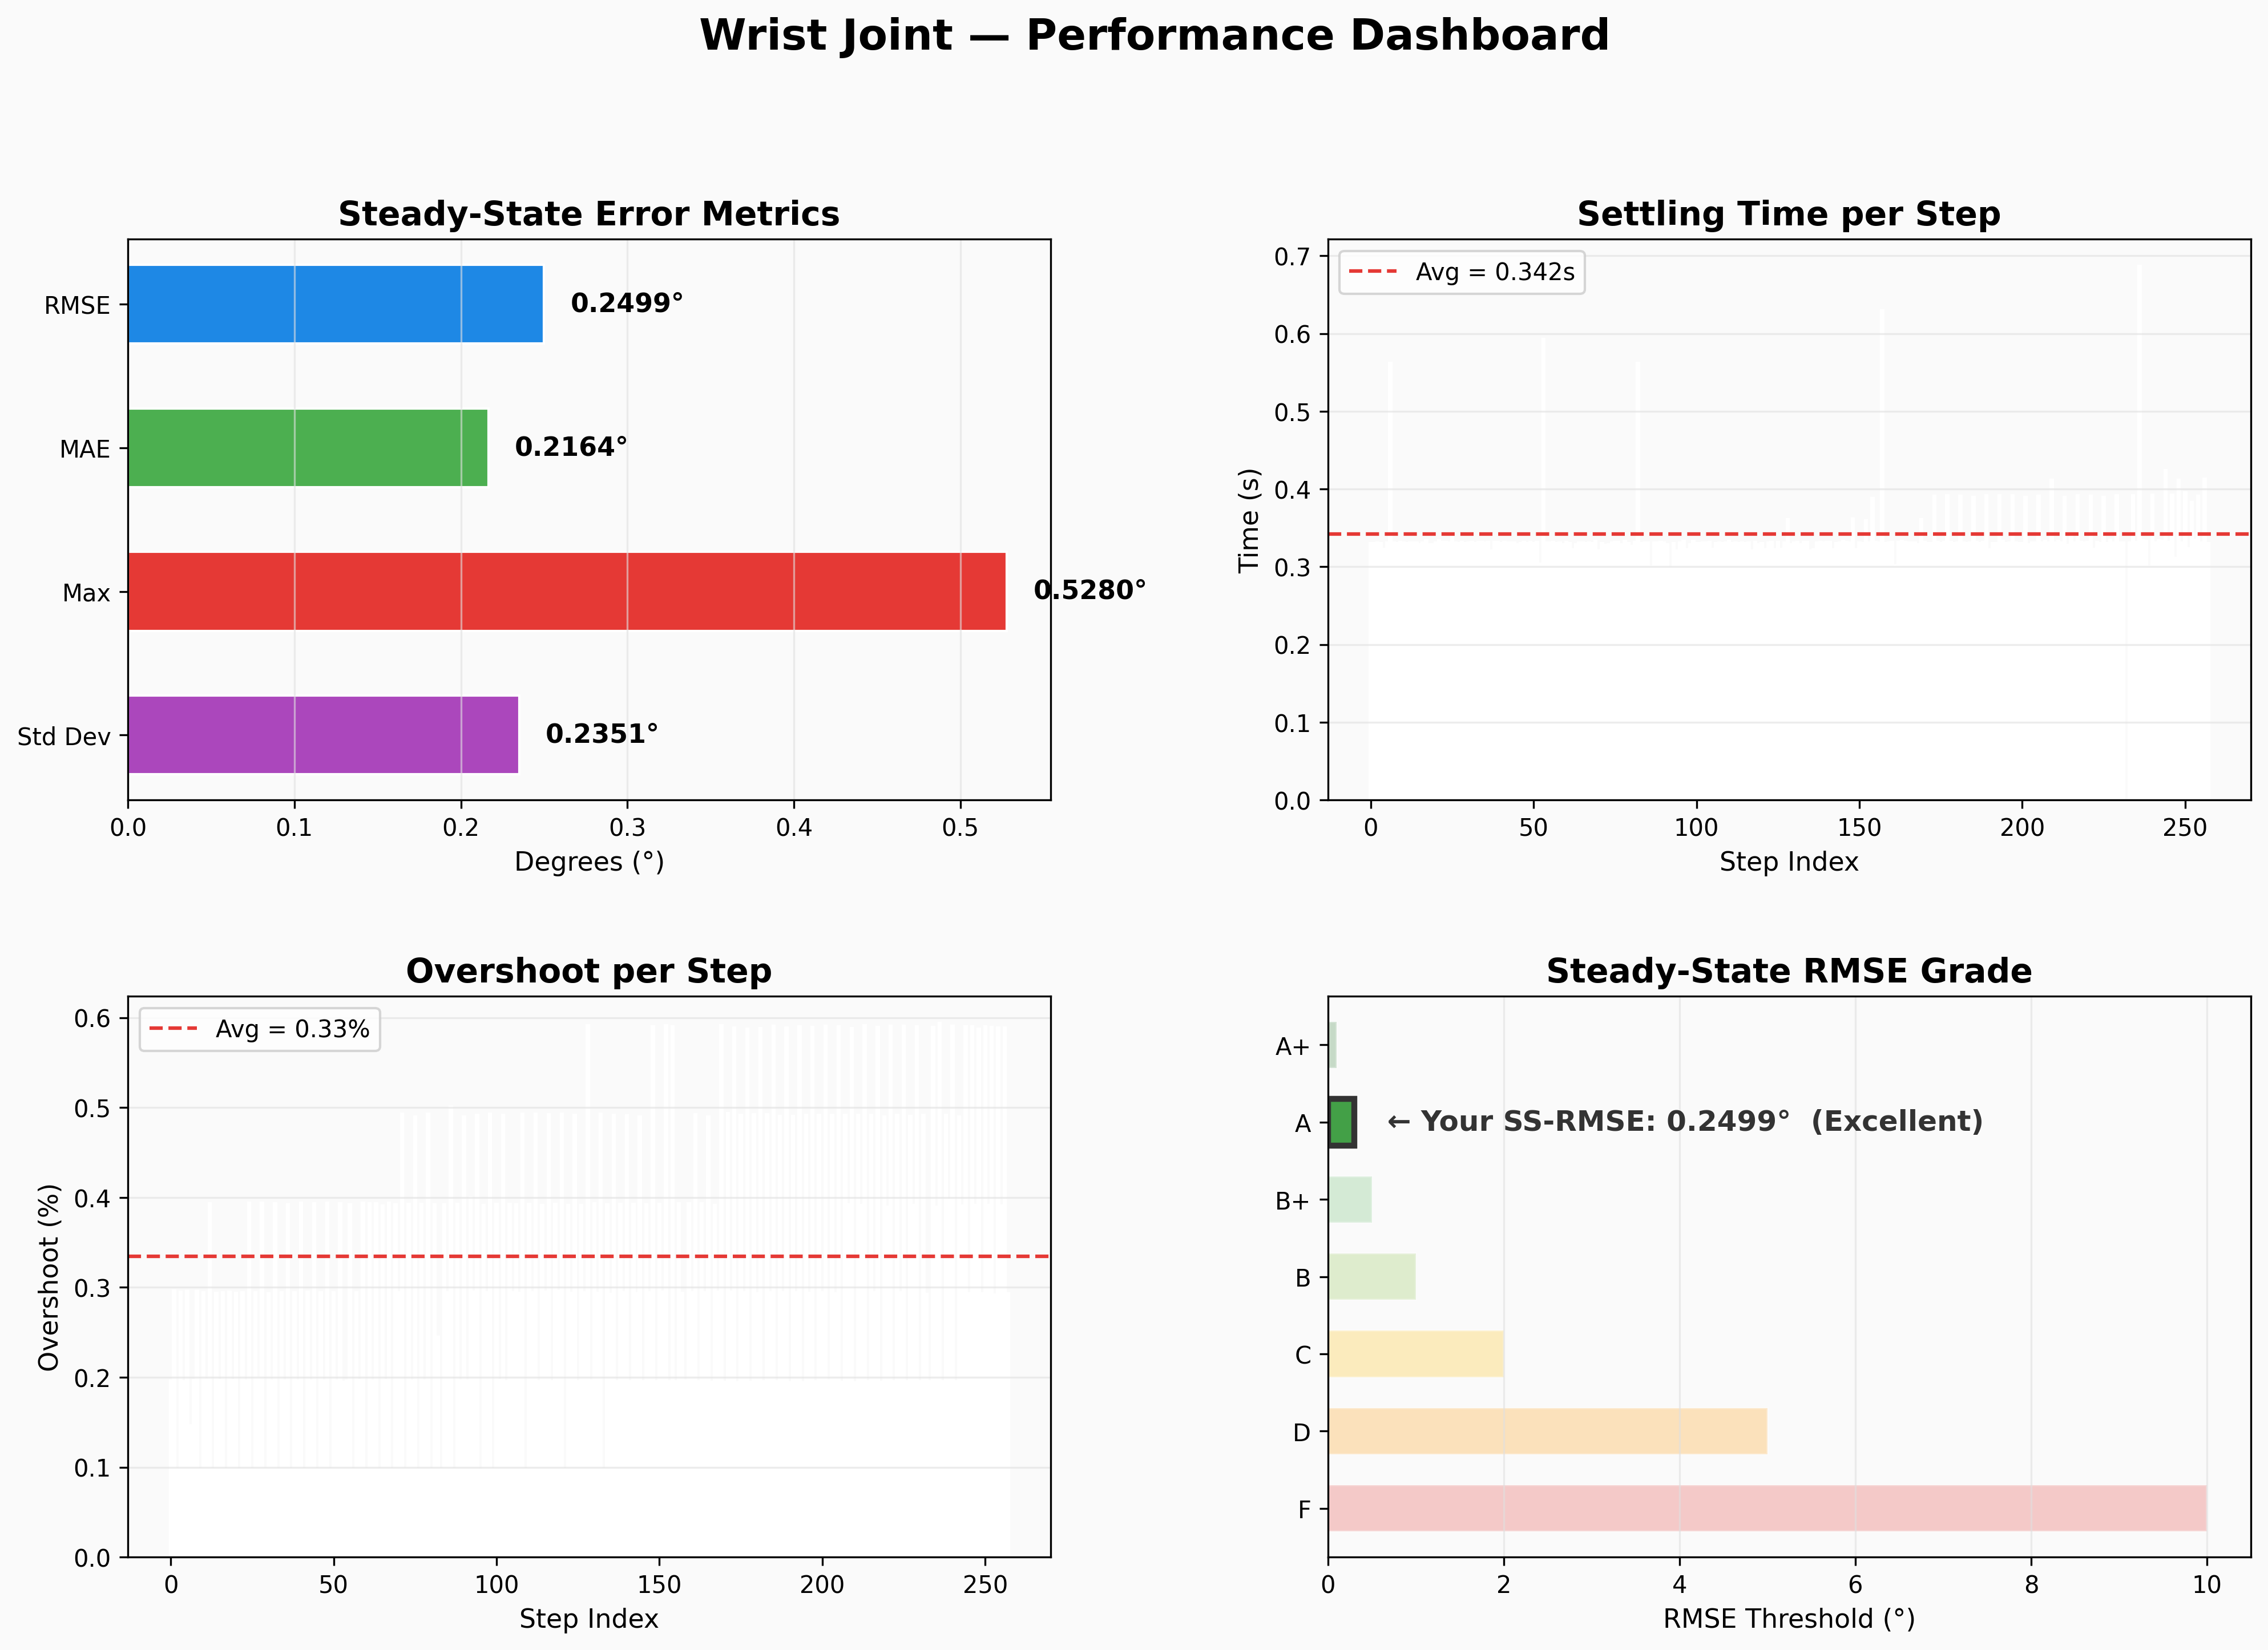
\includegraphics[width=0.8\linewidth]{figures/metric1_0.png}
		}
		\hfill
		\subfloat[Temporal Trends]{%
			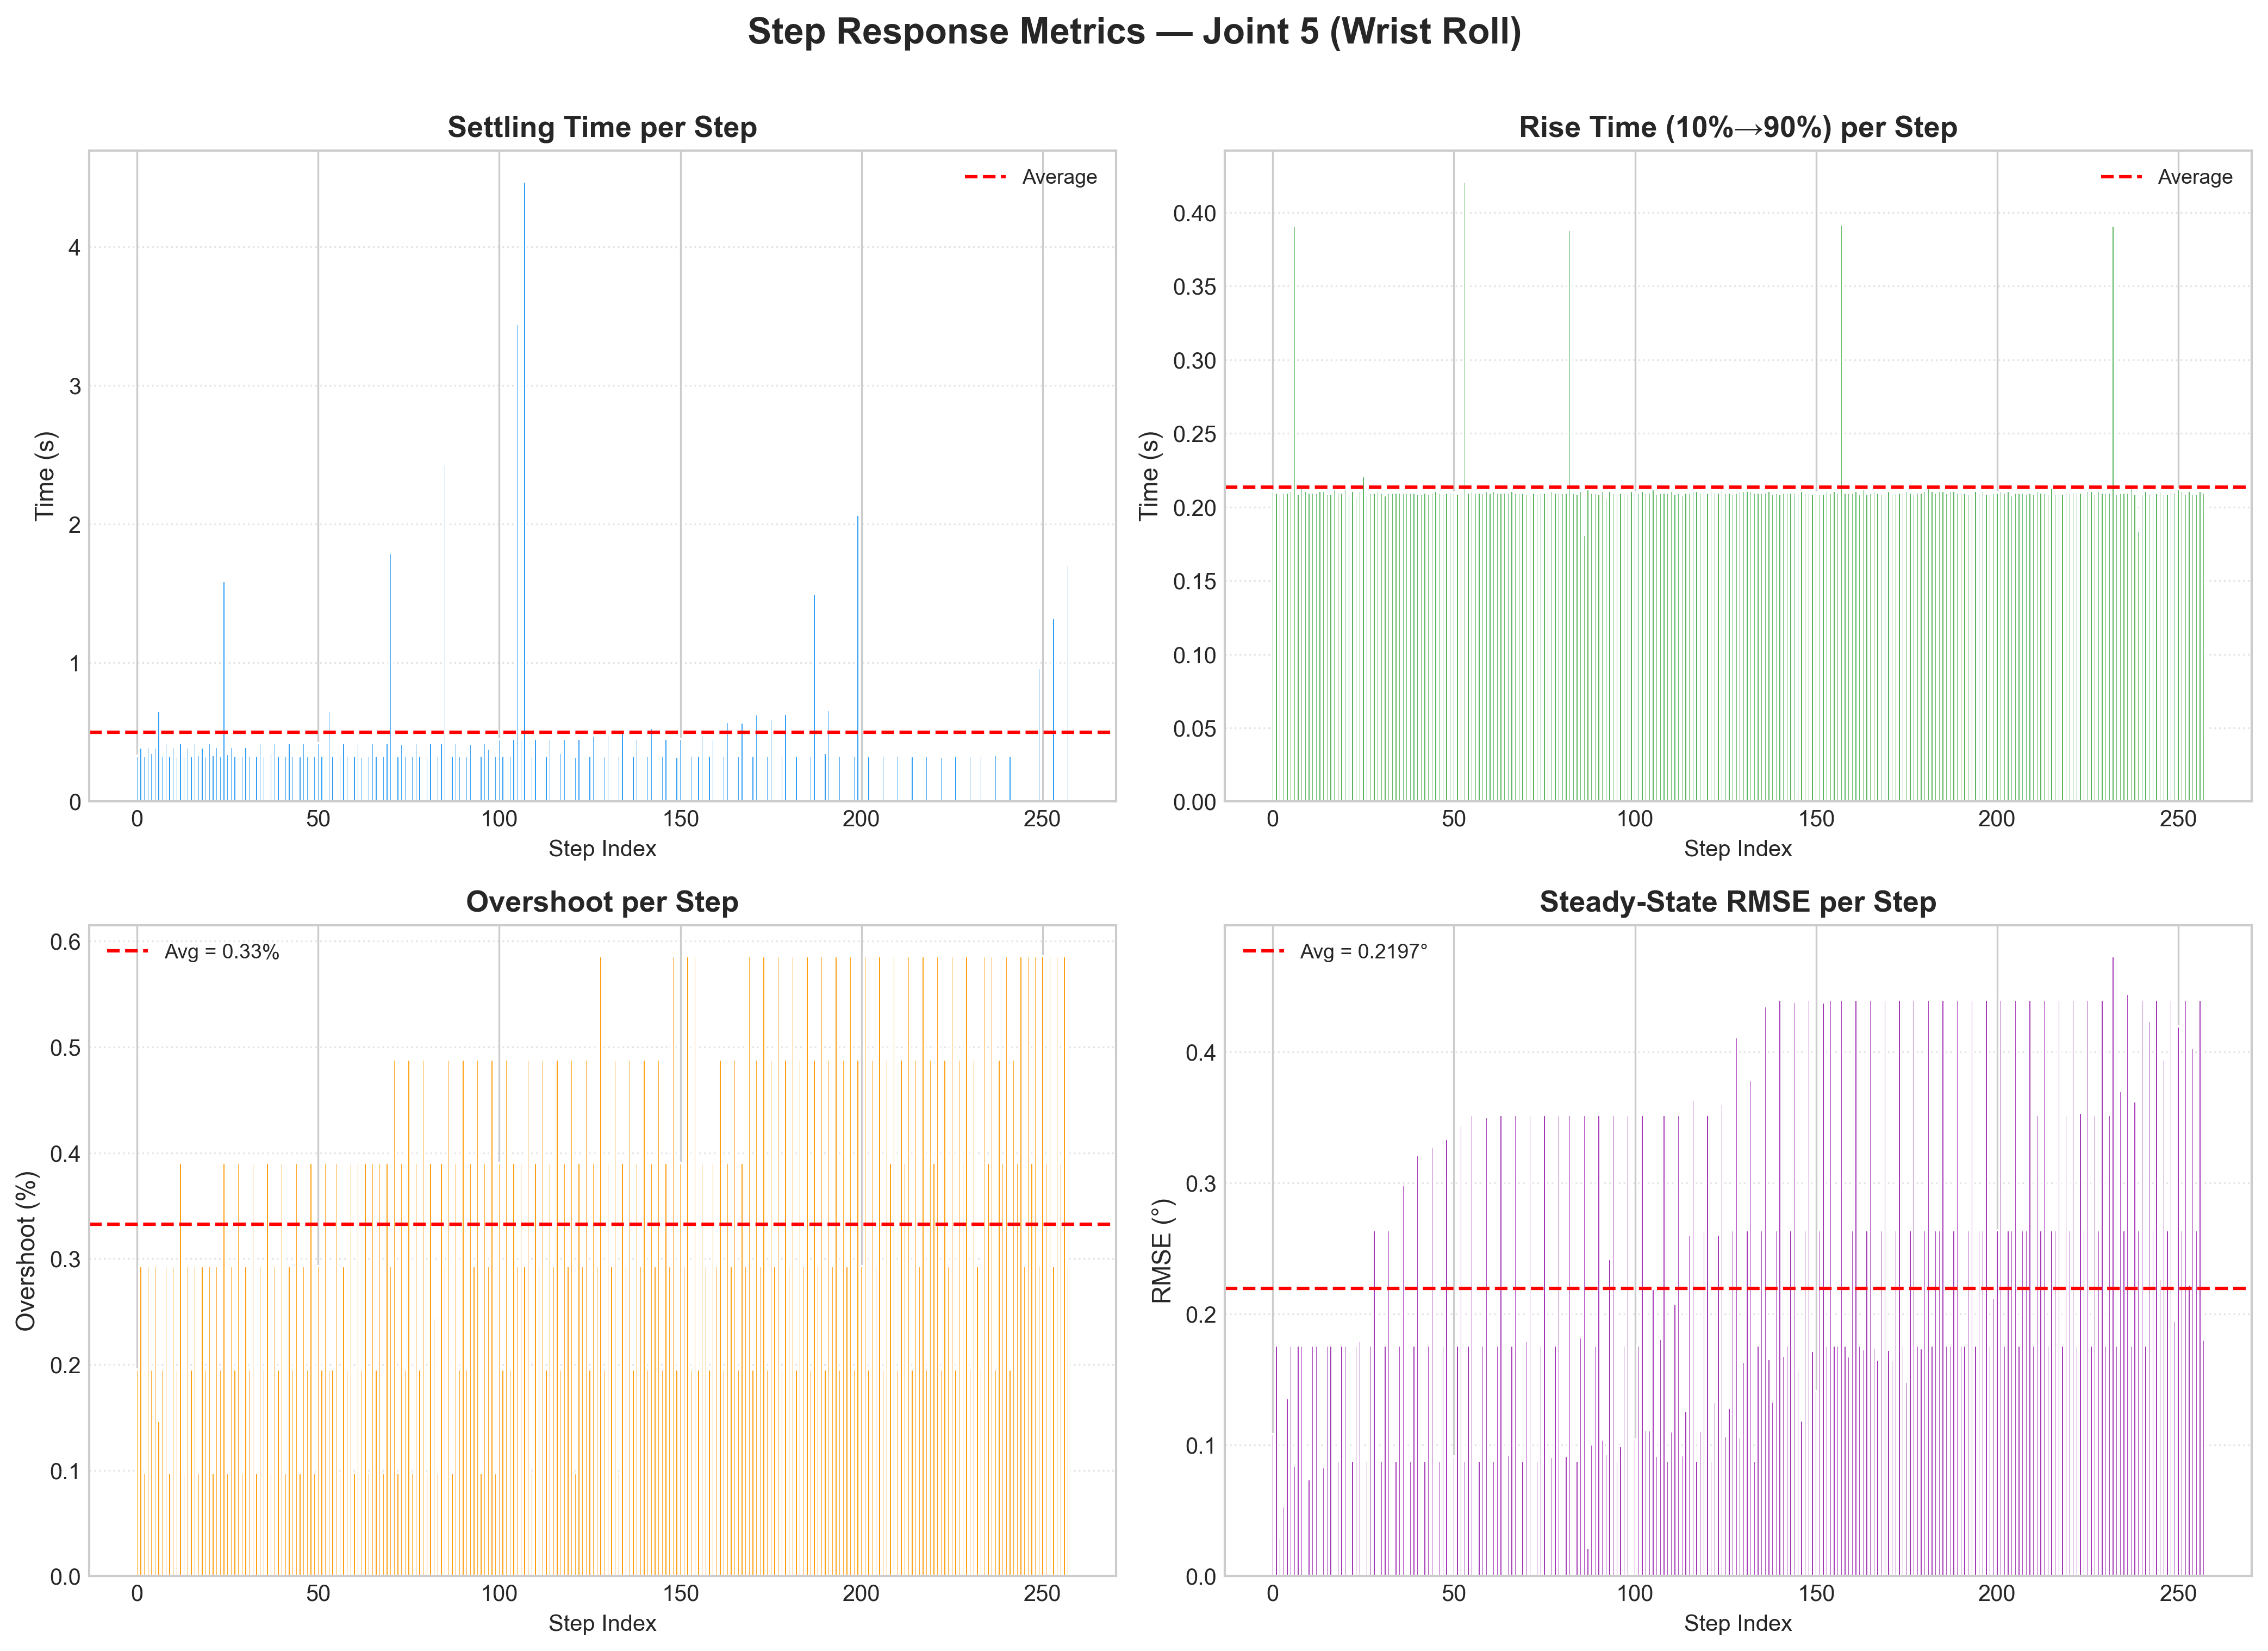
\includegraphics[width=0.8\linewidth]{figures/metric1_1.png}
		}
		\caption{Controller performance and joint tracking accuracy.}
		\label{fig:controller_performance}
	\end{figure}
	
	\textbf{Position accuracy.} Simulation achieves a mean Euclidean
	error of 0.0504\,mm (essentially numerical precision), while the
	physical arm achieves 7.85\,mm mean error with a maximum of 26.6\,mm.
	Under the strict 5\,mm threshold, only 40.0\% of physical executions
	pass, compared to 100\% in simulation. This gap is attributable to
	physical factors absent from the idealised model: joint compliance,
	Dynamixel gear backlash, structural flex under gravity loading, and
	unmodeled friction in the RS-485 daisy-chain transmission.
	
	\textbf{Regional analysis.} Boundary poses achieve a 19.44\% strict
	success rate on physical hardware vs.\ 48.81\% for interior poses.
	Boundary poses impose higher joint torques and more extended
	configurations, amplifying the effect of structural compliance and
	gravity-induced deflection.
	
	\textbf{Orientation fidelity.} 97.5\% of physical executions satisfy
	the $5^\circ$ constraint, with a mean angular error of only
	$1.89^\circ$. Compared to simulation ($0.014^\circ$), the angular
	error is $136\times$ larger in absolute terms, yet it remains
	sub-$2^\circ$ in magnitude and fails the $5^\circ$ threshold for only
	$2.5\%$ of trials. This indicates that \texttt{joint5\_roll} and the
	arm's rotational joints track commanded orientations with substantially
	better fidelity than they achieve Cartesian position.
	
	\textbf{Repeatability.} The mean spatial standard deviation on the
	real arm is $\pm$1.03\,mm. While the absolute value confirms the
	sim-to-real gap, $\pm$1\,mm-class repeatability is broadly consistent
	with published characterizations of Dynamixel-based manipulators at
	similar payload and configuration ranges.
	
	\textbf{Execution time.} The physical arm completes trajectories in
	6.68\,s on average, 2.08\,s faster than simulation. This is expected:
	the simulation includes ROS~2 middleware overhead, trajectory
	interpolation within MoveIt~2, and visualisation updates absent during
	physical execution. The execution-time gap is not a performance
	concern.
	
	\begin{figure}[t]
		\centering
		\subfloat[Heatmap Analysis]{%
			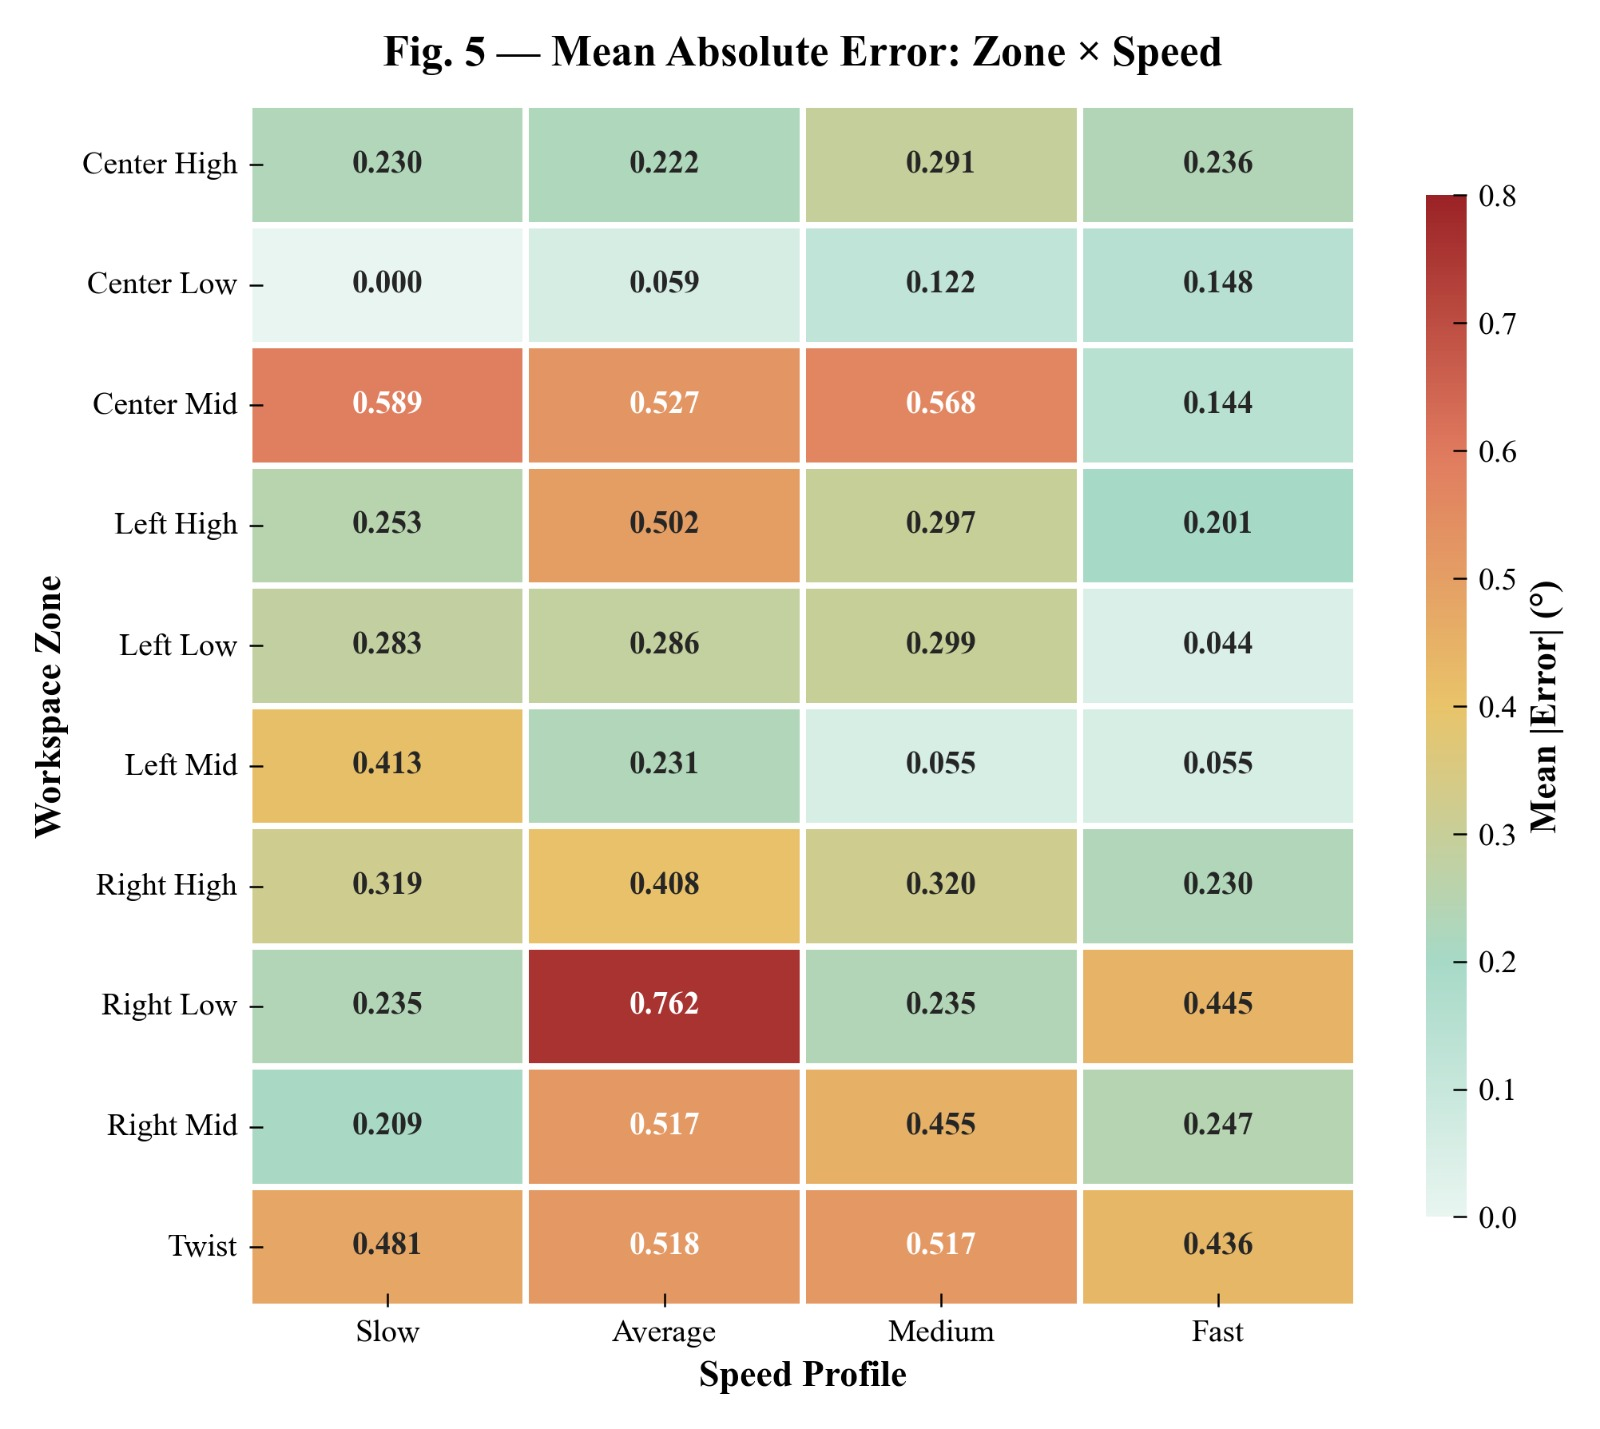
\includegraphics[width=0.32\linewidth]{figures/metric2_0.jpeg}
		}
		\hfill
		\subfloat[Temporal Trends]{%
			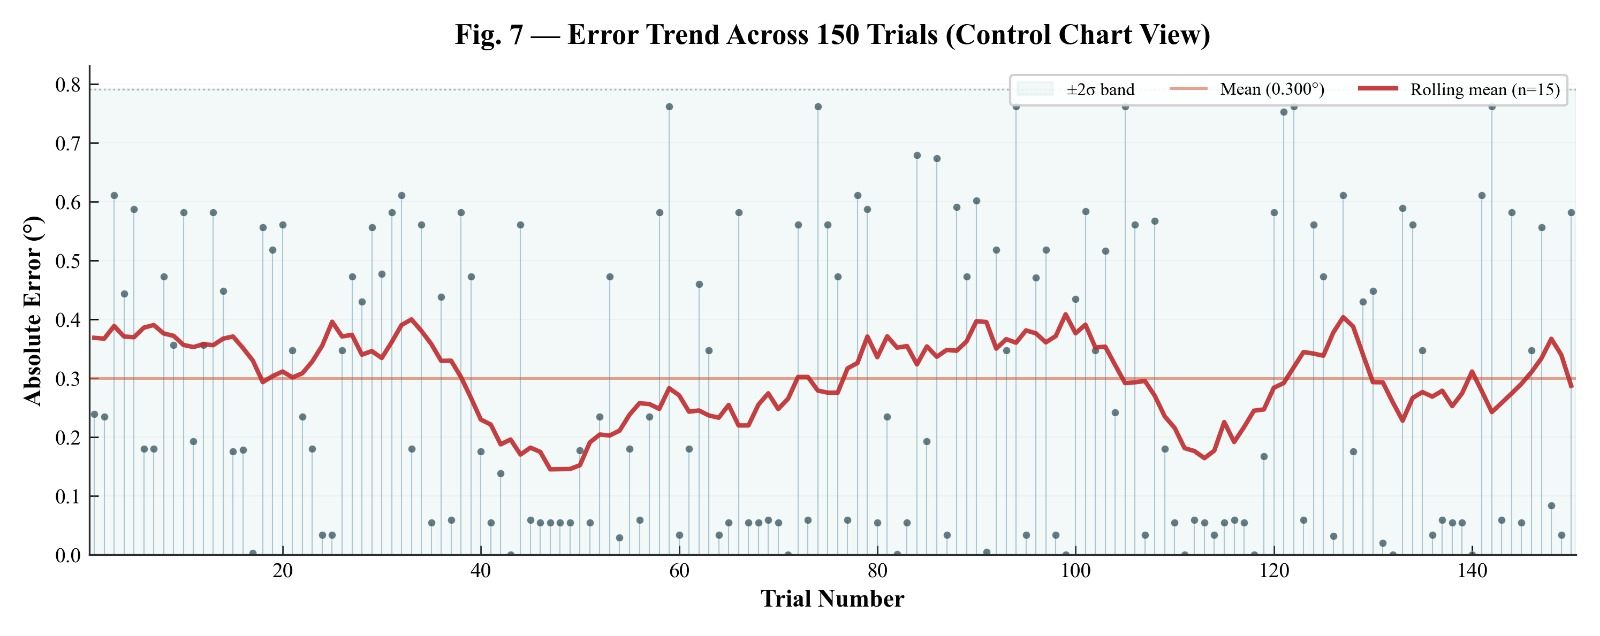
\includegraphics[width=0.32\linewidth]{figures/metric2_1.jpeg}
		}
		\hfill
		\subfloat[Distribution]{%
			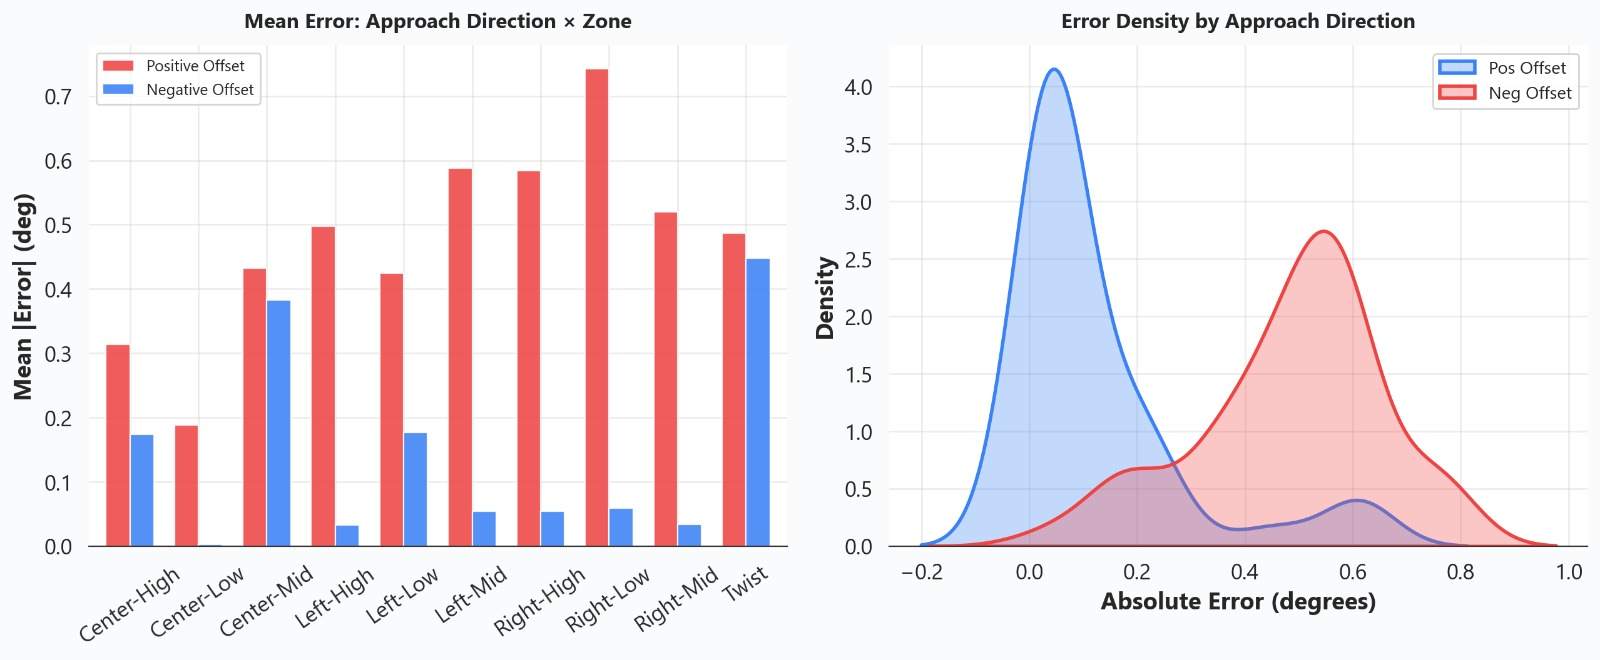
\includegraphics[width=0.32\linewidth]{figures/metric2_2.jpeg}
		}
		\caption{End-effector pose repeatability analysis.}
		\label{fig:repeatability}
	\end{figure}
	
	\begin{figure}[t]
		\centering
		\subfloat[Heatmap Analysis]{%
			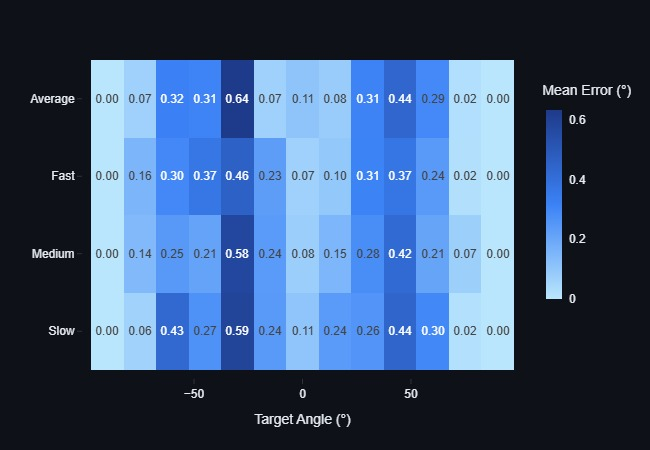
\includegraphics[width=0.32\linewidth]{figures/metric3_0.jpeg}
		}
		\hfill
		\subfloat[Temporal Trends]{%
			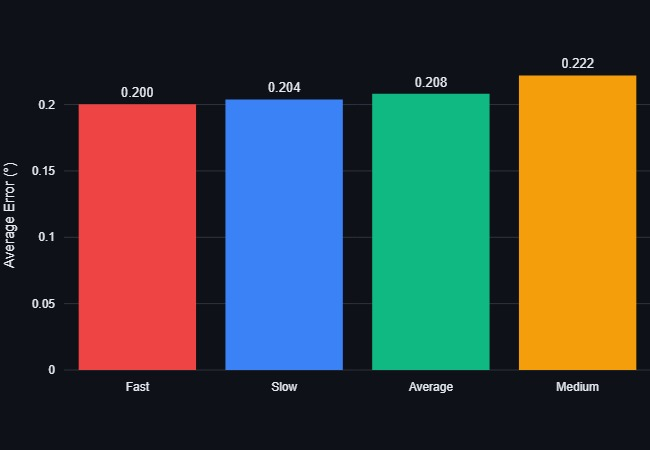
\includegraphics[width=0.32\linewidth]{figures/metric3_1.jpeg}
		}
		\hfill
		\subfloat[Distribution]{%
			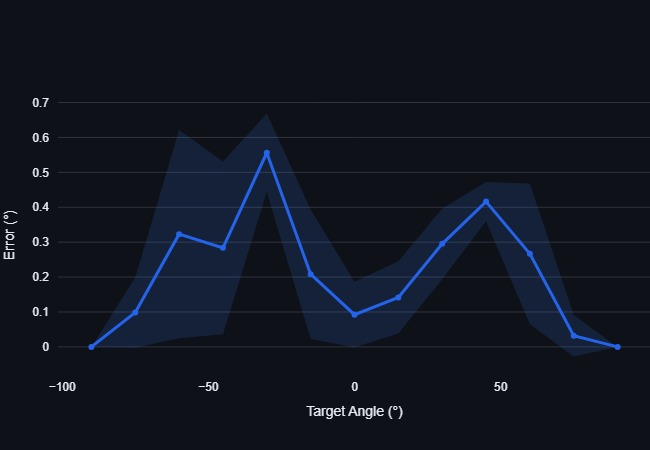
\includegraphics[width=0.32\linewidth]{figures/metric3_2.jpeg}
		}
		
		\vspace{4pt}
		
		\subfloat[Heatmap (grouped)]{%
			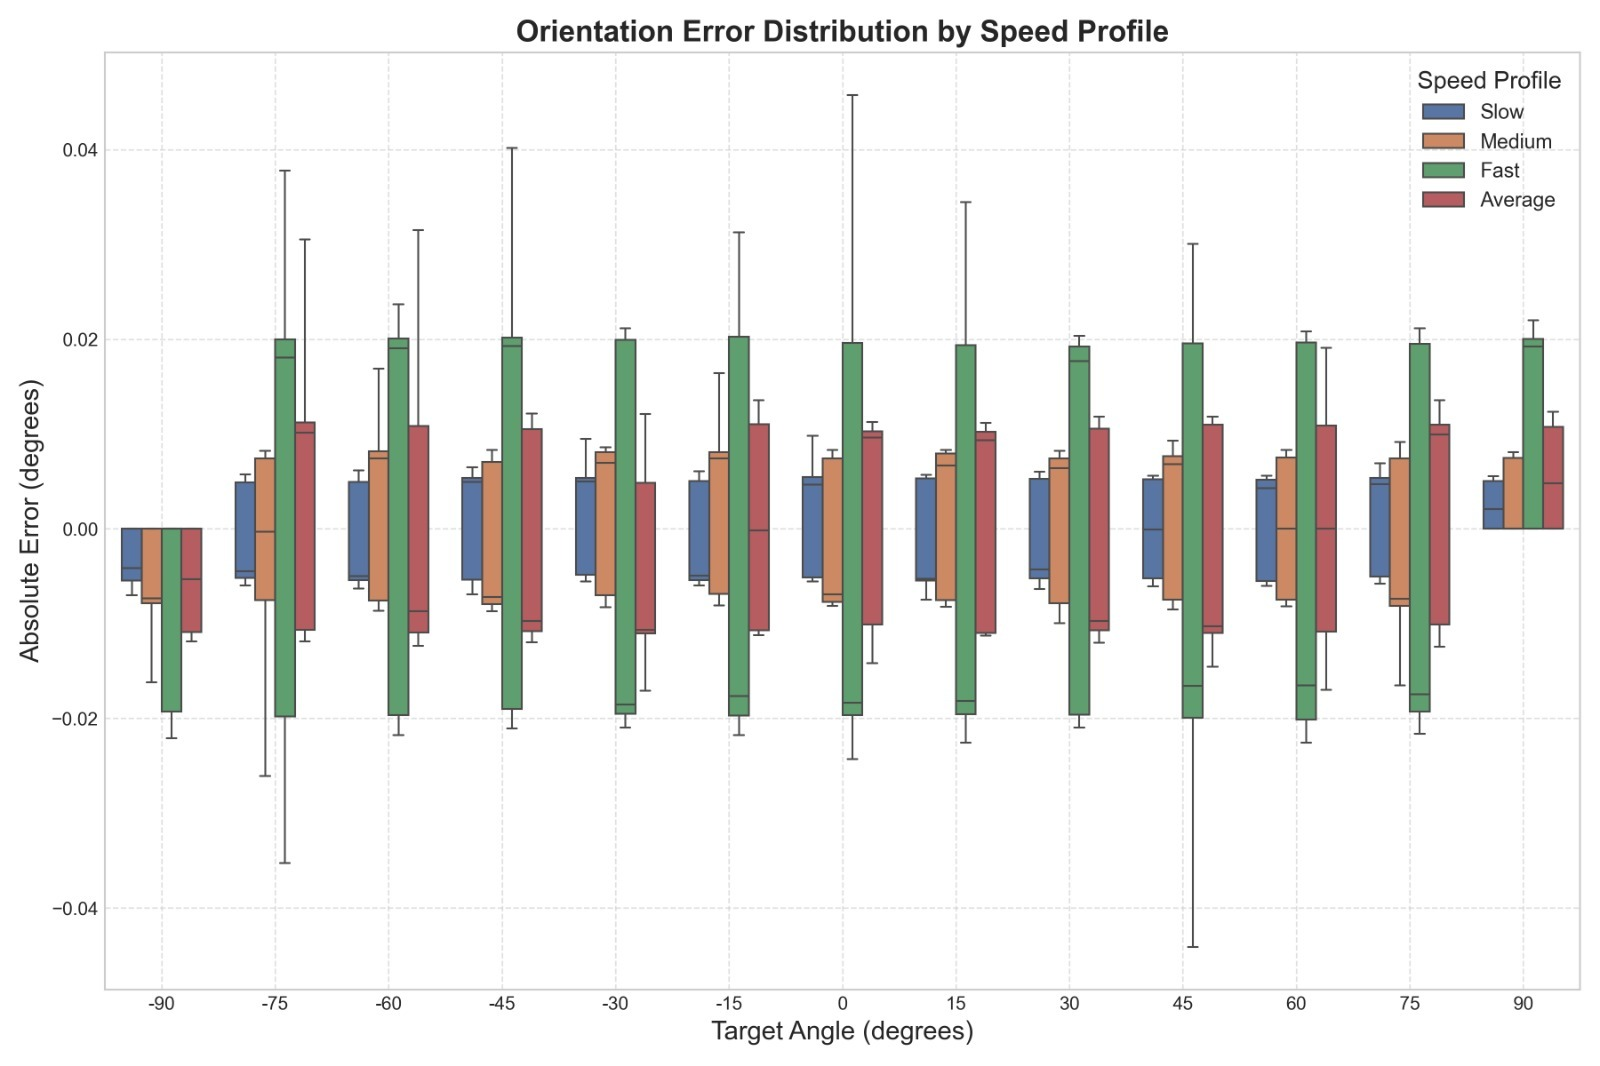
\includegraphics[width=0.47\linewidth]{figures/metric3g_0.jpeg}
		}
		\hfill
		\subfloat[Trends (grouped)]{%
			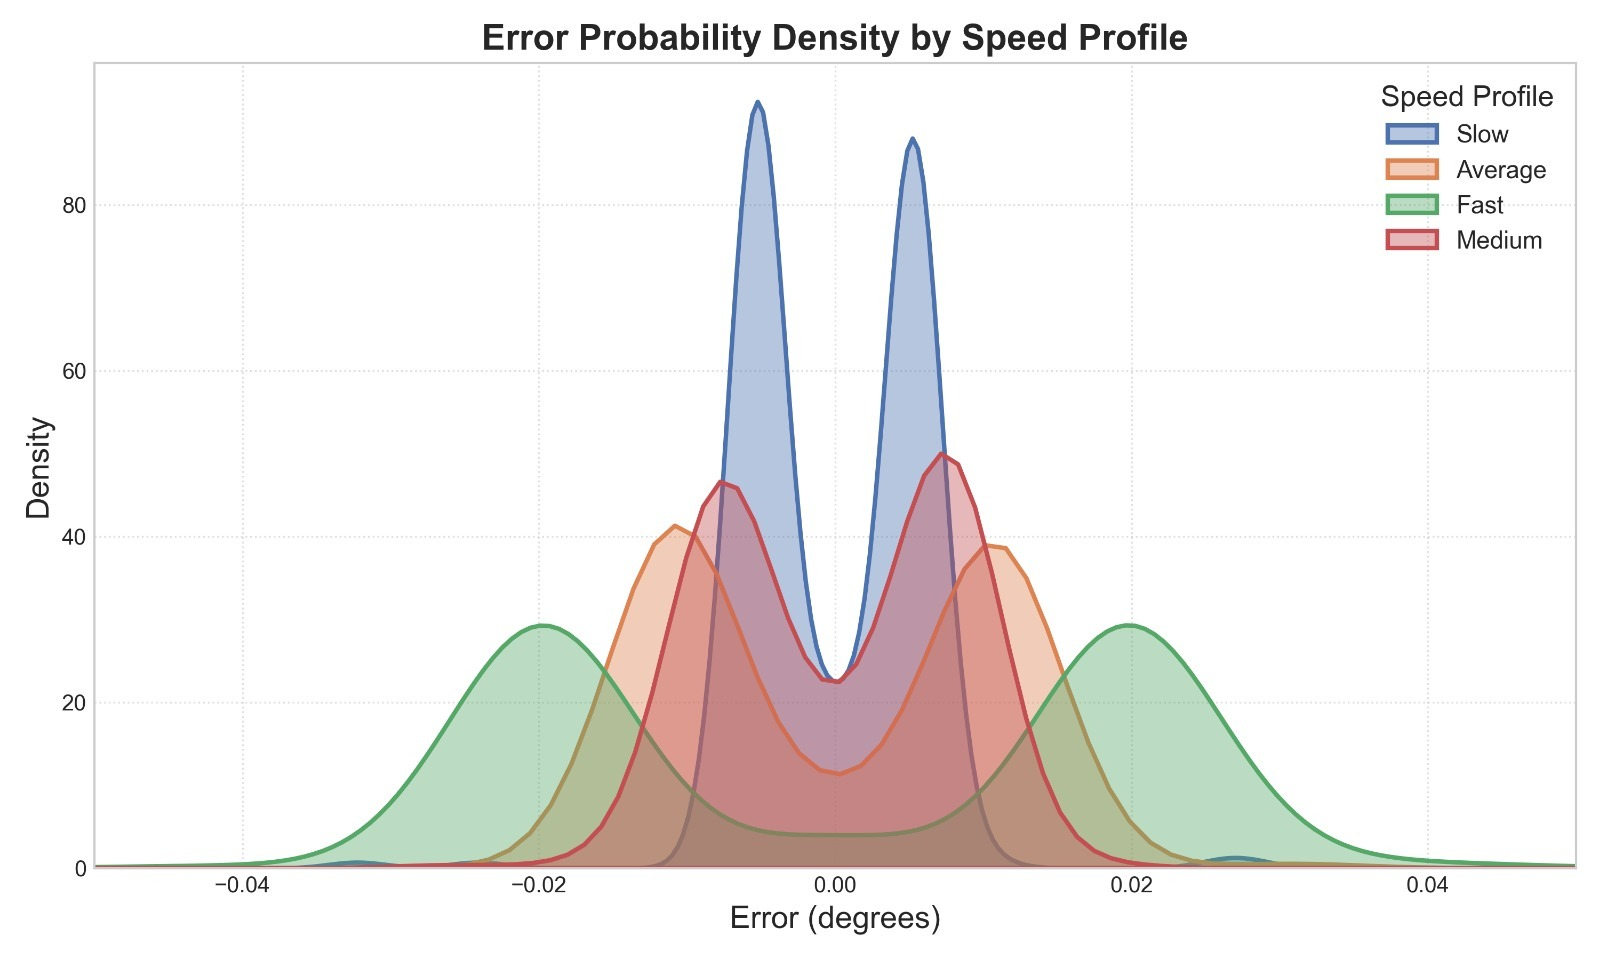
\includegraphics[width=0.47\linewidth]{figures/metric3g_1.jpeg}
		}
		\caption{Orientational fidelity analysis.}
		\label{fig:orientation_quality}
	\end{figure}
	
	\subsection{Summary of Quantitative Outcomes}
	
	Table~\ref{tab:summary} consolidates all primary quantitative results
	--- simulation benchmarks and hardware validation --- for direct
	reference.
	
	\begin{table*}[t]
		\centering
		\caption{Complete Summary of Quantitative Results}
		\label{tab:summary}
		\renewcommand{\arraystretch}{1.3}
		\small
		\begin{tabular}{llll}
			\toprule
			\textbf{Metric} & \textbf{5-DOF (Joint Removed)} & \textbf{6-DOF (Full)} & \textbf{Note} \\
			\midrule
			\multicolumn{4}{l}{\textit{Simulation --- Kinematic and Planning}} \\
			IK feasibility (7 orientations)              & 1/7 (14.3\%)    & 7/7 (100\%)          & Structurally exact \\
			Cross-config.\ IK (6-DOF $\to$ 5-DOF)       & 0/7239 (0.0\%)  & ---                  & 100\% dexterity expansion \\
			Planning success (initial)                   & 0/10 (0.0\%)    & 21/70 (30.0\%)       & $\chi^2=4.2$, $p=0.04$ \\
			Planning success (refined)                   & 0/70 (0.0\%)    & 28/112 (25.0\%)      & $\chi^2=18.81$, $p<0.00002$ \\
			Planning 95\% CI                             & 0.0\%--5.2\%    & 17.9\%--33.8\%       & Non-overlapping \\
			Cramer's $V$                                 & \multicolumn{2}{l}{0.321 (medium-to-large)} & --- \\
			Cohen's $h$                                  & \multicolumn{2}{l}{1.107 (large, $h>0.8$)}  & --- \\
			Orientation coverage                         & $0^\circ$ only  & Full $\pm180^\circ$  & --- \\
			\midrule
			\multicolumn{4}{l}{\textit{Hardware Validation --- 6-DOF Physical Arm (120 poses)}} \\
			Planning feasibility                         & ---  & 100.0\%        & Sim and real \\
			Strict position success ($<$5\,mm)           & ---  & 40.0\%         & Real; 100\% in sim \\
			Orientation success ($<$5$^\circ$)           & ---  & 97.5\%         & Real; 100\% in sim \\
			Mean Cartesian error                         & ---  & 7.85\,mm       & Real; 0.05\,mm in sim \\
			Repeatability ($\sigma$)                     & ---  & $\pm$1.03\,mm  & Real; $\pm$0.006\,mm in sim \\
			Mean angular error                           & ---  & $1.89^\circ$   & Real; $0.014^\circ$ in sim \\
			\bottomrule
		\end{tabular}
	\end{table*}
	
	
	% ============================================================
	\section{Discussion}
	\label{sec:discussion}
	% ============================================================
	
	\subsection{Three Complementary Lines of Evidence}
	
	The results deliver a consistent conclusion through three independent
	lines of evidence.
	
	\textbf{Kinematic evidence.}
	The IK feasibility results (Table~\ref{tab:ik_results}) demonstrate a
	$7\times$ improvement in orientation coverage (1/7 $\rightarrow$ 7/7).
	This is an exact, planner-independent result: the absence of a
	wrist-roll joint imposes a hard mathematical constraint on the 5-DOF IK
	solution manifold. No algorithm can overcome it.
	
	\textbf{Planning evidence.}
	The improvement from 0.0\% to 25.0--30.0\% planning success in the
	constrained corridor translates the kinematic advantage into a
	task-level benefit. Crucially, even the $0^\circ$-roll goal --- the
	only one the 5-DOF arm can reach --- yields 0\% planning success for
	the 5-DOF arm in the corridor. The failure is geometric, not kinematic.
	
	\textbf{Statistical evidence.}
	The chi-square test ($\chi^2(1) = 18.81$, $p = 1.4\times10^{-5}$) and
	effect sizes (Cramer's $V = 0.321$, Cohen's $h = 1.107$) confirm the
	performance gap is not a sampling artifact. Non-overlapping 95\% CIs
	provide additional visual confirmation.
	
	\subsection{The Role of Wrist-Roll Redundancy}
	
	Planning success for the 6-DOF arm peaks at the most demanding
	orientations ($60^\circ$--$90^\circ$, 60--80\% per goal) and is zero
	at the simplest ($0^\circ$--$45^\circ$). This counter-intuitive pattern
	reflects corridor geometry: at high roll angles, \texttt{joint5\_roll}
	aligns the gripper approximately parallel to the corridor walls,
	reducing the effective distal cross-section and opening collision-free
	approach trajectories that are geometrically blocked when the gripper
	is perpendicular to the walls. This result articulates a broader
	principle: the practical value of kinematic redundancy is task- and
	environment-specific. It is highest precisely where the baseline system
	has no alternative approach geometry available.
	
	\subsection{Dexterity Expansion and Kinematic Separability}
	
	The cross-configuration test (Table~\ref{tab:cross_config}) yields a
	shared kinematic space of 0\% and dexterity expansion of 100\%: the
	6-DOF and 5-DOF feasible manifolds are entirely disjoint in the
	evaluated orientation space. Adding the wrist-roll joint expands the
	reachable orientation manifold to include non-zero-roll poses, which
	are structurally unreachable by the 5-DOF configuration; the
	cross-configuration test (Table~\ref{tab:cross_config}) confirms this
	expansion empirically. Within the tested orientation and corridor
	conditions, the retrofit expands the feasible task space rather than
	incrementally improving performance on an already-shared task set.
	
	\subsection{Sim-to-Real Analysis}
	\label{sec:sim_to_real}
	
	The hardware validation results (Table~\ref{tab:hw_comparison}) reveal
	a nuanced sim-to-real profile that distinguishes between position
	accuracy and orientation fidelity.
	
	\textbf{Position accuracy gap is significant.}
	The mean Cartesian error increases from 0.05\,mm in simulation to
	7.85\,mm on the physical arm --- a factor of $\sim$156. Under the
	5\,mm strict threshold, the physical success rate falls from 100\% to
	40.0\%. The primary contributors are Dynamixel gear backlash and
	structural compliance that accumulate along the kinematic chain,
	particularly under gravity loading at extended configurations.
	Boundary poses, which impose higher joint torques, show substantially
	lower success rates (19.44\%) than interior poses (48.81\%),
	consistent with this interpretation.
	
	\textbf{Orientation fidelity is preserved.}
	Despite the position accuracy gap, 97.5\% of physical executions
	satisfy the $5^\circ$ orientation constraint, with a mean angular
	error of $1.89^\circ$. Orientation is controlled primarily by
	\texttt{joint5\_roll} (a compact, low-inertia distal joint) and the
	distal wrist joints, which carry less load and exhibit less compliance
	than the proximal shoulder and elbow joints. The mechanical advantage
	of the distal position insulates rotational control from the compliance
	effects that dominate position error.
	
	\textbf{Repeatability is adequate.}
	The $\pm$1.03\,mm spatial standard deviation on the physical arm,
	while $\sim$188$\times$ larger than in simulation, falls within the
	commonly accepted repeatability range for Dynamixel-based platforms of
	comparable scale. It is sufficient for tasks where orientation
	alignment matters more than sub-millimetre Cartesian precision.
	
	\textbf{Execution time.}
	The physical arm completes trajectories 2.08\,s faster on average than
	the simulation (6.68\,s vs.\ 8.76\,s). This gap arises from ROS~2
	middleware, visualisation, and trajectory interpolation overhead
	present in simulation but not on hardware, and does not reflect a
	real-world performance advantage.
	
	\textbf{Summary of the sim-to-real gap.}
	The gap is real and non-trivial for position accuracy; it is
	acceptable for orientation accuracy. For applications where the primary
	benefit of the 6-DOF retrofit is orientation freedom --- the stated
	purpose of this work --- the physical arm delivers the capability at an
	operationally useful level (97.5\% orientation success, $1.89^\circ$
	mean error).
	
	\subsection{Practical Implications for Low-Cost Manipulator Design}
	
	\textit{Within the evaluated orientation-reachability and
		corridor-planning benchmarks, the additional DOF determines whether
		the tested goals are reachable at all, rather than merely improving
		performance on goals reachable by both configurations.}
	Extending this finding to concrete manipulation tasks (e.g., insertion,
	cap alignment) is left to future work.
	
	\textit{Orientation and position are decoupled in practice.}
	The hardware results demonstrate that the wrist-roll joint delivers its
	primary benefit --- orientation control --- with high fidelity even
	when absolute Cartesian position accuracy is limited by platform
	compliance.
	
	\textit{Low cost and high capability are compatible.}
	The total hardware addition costs approximately 5,599\,INR
	($<$\$70\,USD), both mechanical adapters are 3D-printable, and
	assembly requires approximately one hour. This yields a $7\times$
	expansion in orientation coverage under the tested protocol, suggesting
	feasibility for orientation-constrained task classes (e.g., insertion,
	alignment) that remain to be directly validated.
	
	\textit{Reproducibility requires a full stack.}
	This work provides URDF/Xacro, \texttt{ros2\_control}, MoveIt~2, GUI,
	and benchmarking scripts as open artifacts, enabling other laboratories
	to replicate both the retrofit and its evaluation with minimal
	incremental effort.
	
	\subsection{Future Work}
	
	\begin{itemize}
		\item \textbf{Closed-loop Cartesian control}: Incorporating a
		Cartesian position feedback loop --- via visual markers or a
		force-torque sensor --- to reduce the physical position error
		from $\sim$7.9\,mm toward the $<$5\,mm target across all
		workspace regions.
		
		\item \textbf{Roll-critical task evaluation}: Benchmarking on
		tasks that inherently require wrist roll (tube insertion, cap
		alignment, bolt rotation) to demonstrate operational benefit
		beyond corridor navigation.
		
		\item \textbf{Multi-planner benchmarking}: Extension of the
		MoveIt~2 Benchmark Suite runs to PRM*, LazyPRM, and LBKPIECE
		to characterise planning improvement across the full planner
		landscape.
		
		\item \textbf{Learning pipeline integration}: Integration with
		imitation learning or reinforcement learning pipelines to
		demonstrate that the richer $SO(2)$ roll action space enables
		more capable manipulation policies.
		
	\end{itemize}
	
	
	% ============================================================
	\section{Conclusion}
	\label{sec:conclusion}
	% ============================================================
	
	This work presented a systematic retrofit of a 5-DOF manipulator into
	a 6-DOF system and evaluated its impact through kinematic analysis,
	motion planning benchmarks, and real-world validation. The results
	demonstrate that the addition of a wrist-roll joint leads to an
	expansion of the reachable orientation space, with cross-configuration
	analysis revealing a complete absence of shared kinematic solutions
	between the two configurations under the evaluated orientation protocol.
	
	The observed gains reflect an expansion in kinematic expressiveness
	rather than an incremental performance improvement, indicating
	feasibility for orientation-constrained goals that are structurally
	infeasible for the 5-DOF system. These findings illustrate the role
	of kinematic completeness in constrained manipulation scenarios and
	motivate further evaluation on concrete task-level benchmarks.
	
	Future work will explore dynamic task execution, optimization of
	planning strategies, and deployment in more complex real-world
	environments.
	
	
	\bibliographystyle{IEEEtran}
	\bibliography{references2}
	
\end{document}